% ==================================================================
% TEMPLATE TCC MACKENZIE - BRUNO GASPARONI BALLERINI
% Baseado nas normas do Guia do TCC 2022 - Universidade Presbiteriana Mackenzie
% ==================================================================

\documentclass[12pt,a4paper,oneside]{report}

% ==================================================================
% PACOTES NECESSÁRIOS
% ==================================================================
\usepackage[utf8]{inputenc}
\usepackage[T1]{fontenc}
\usepackage[portuguese]{babel}
\usepackage{mathptmx} % Times New Roman
\usepackage{setspace}
\usepackage{geometry}
\usepackage{titlesec}
\usepackage{tocloft}
\usepackage{fancyhdr}
\usepackage{graphicx}
\usepackage{amsmath}
\usepackage{amsfonts}
\usepackage{amssymb}
\usepackage{indentfirst}
\usepackage{caption}
\usepackage{subcaption}
\usepackage{float}
\usepackage[hidelinks]{hyperref}
\usepackage{url}
\usepackage{booktabs}
\usepackage{array}
\usepackage{multirow}
\usepackage{longtable}

% ==================================================================
% CONFIGURAÇÕES GERAIS MACKENZIE
% ==================================================================

% Margens: 3cm (superior e esquerda), 2cm (inferior e direita)
\geometry{
    a4paper,
    top=3cm,
    left=3cm,
    bottom=2cm,
    right=2cm
}

% Espaçamento 1.5
\onehalfspacing

% Recuo de parágrafo 1,25cm
\setlength{\parindent}{1.25cm}

% Espaçamento entre parágrafos - SEM espaço extra (conforme guia p.40)
\setlength{\parskip}{0pt}

% ==================================================================
% CONFIGURAÇÃO DE TÍTULOS (NORMAS MACKENZIE)
% ==================================================================

% Seção primária: 1 LETRAS MAIÚSCULAS EM NEGRITO  
\titleformat{\chapter}[hang]
{\normalfont\fontsize{12}{14.4}\bfseries}
{\thechapter}{1em}{\MakeUppercase}
\titlespacing*{\chapter}{0pt}{0pt}{12pt}

% Títulos de capítulos não numerados (centralizados)
\titleformat{name=\chapter,numberless}[block]
{\normalfont\fontsize{12}{14.4}\bfseries\centering}
{}{0pt}{\MakeUppercase}
\titlespacing*{name=\chapter,numberless}{0pt}{0pt}{12pt}

% Seção secundária: 1.1 LETRAS MAIÚSCULAS SEM NEGRITO
\titleformat{\section}[hang]
{\normalfont\fontsize{12}{14.4}}
{\thesection}{1em}{\MakeUppercase}
\titlespacing*{\section}{0pt}{\baselineskip}{\baselineskip}

% Seção terciária: 1.1.1 Letras minúsculas em negrito
\titleformat{\subsection}[hang]
{\normalfont\fontsize{12}{14.4}\bfseries}
{\thesubsection}{1em}{}
\titlespacing*{\subsection}{0pt}{12pt}{12pt}

% Seção quaternária: 1.1.1.1 Letras minúsculas sem negrito
\titleformat{\subsubsection}[hang]
{\normalfont\fontsize{12}{14.4}}
{\thesubsubsection}{1em}{}
\titlespacing*{\subsubsection}{0pt}{12pt}{12pt}

% Seção quinária: 1.1.1.1.1 Letras minúsculas em itálico
\titleformat{\paragraph}[hang]
{\normalfont\fontsize{12}{14.4}\itshape}
{\theparagraph}{1em}{}
\titlespacing*{\paragraph}{0pt}{12pt}{12pt}

% ==================================================================
% NUMERAÇÃO DE PÁGINAS
% ==================================================================
\setlength{\headheight}{13.19998pt}
\pagestyle{fancy}
\fancyhf{}
% Numeração a 2cm das bordas superior e direita
\fancyhead[R]{\fontsize{11}{13.2}\selectfont\thepage}
\fancyheadoffset{0cm}
\renewcommand{\headrulewidth}{0pt}

% ==================================================================
% CONFIGURAÇÃO DO SUMÁRIO
% ==================================================================
\renewcommand{\contentsname}{SUMÁRIO}
\renewcommand{\cftchapfont}{\fontsize{12}{14.4}\selectfont\bfseries}
\renewcommand{\cftsecfont}{\fontsize{12}{14.4}\selectfont}
\renewcommand{\cftsubsecfont}{\fontsize{12}{14.4}\selectfont}
\renewcommand{\cftchapleader}{\cftdotfill{\cftdotsep}}
\setlength{\cftbeforechapskip}{6pt}

% ==================================================================
% INÍCIO DO DOCUMENTO
% ==================================================================
\begin{document}

% CAPA - sem numeração
\pagenumbering{gobble}
% ==================================================================
% CAPA - CONFORME MODELO MACKENZIE (Apêndice D do Guia)
% ==================================================================

\thispagestyle{empty}

\begin{center}

% Espaçamento superior
\vspace*{3cm}

% Nome da instituição
{\fontsize{12}{14.4}\selectfont\bfseries\MakeUppercase{UNIVERSIDADE PRESBITERIANA MACKENZIE}}\\[0.8cm]
{\fontsize{12}{14.4}\selectfont\bfseries\MakeUppercase{Centro de Ciências e Tecnologia – CCT}}\\[0.5cm]
{\fontsize{12}{14.4}\selectfont\bfseries\MakeUppercase{Curso de Engenharia de Produção}}

\vspace{5cm}

% Nome do autor
{\fontsize{12}{14.4}\selectfont\bfseries\MakeUppercase{BRUNO GASPARONI BALLERINI}}

\vspace{5cm}

% Título do trabalho
{\fontsize{12}{14.4}\selectfont\bfseries\MakeUppercase{%
COMPARAÇÃO ENTRE MÉTODOS DE ALOCAÇÃO DE CARTEIRAS:\\[0.3cm]
MARKOWITZ, EQUAL WEIGHT E RISK PARITY\\[0.3cm] 
NO MERCADO BRASILEIRO (2018–2019)%
}}

\vfill

% Local e ano
{\fontsize{12}{14.4}\selectfont
Campinas\\[0.3cm]
2025}

\end{center}
\newpage

% FOLHA DE ROSTO - inicia contagem (página 1, mas não aparece)
\pagenumbering{arabic}
\setcounter{page}{1}
\thispagestyle{empty}
% ==================================================================
% FOLHA DE ROSTO - CONFORME MODELO MACKENZIE (Apêndice E do Guia)
% ==================================================================

\thispagestyle{empty}

\begin{center}

\vspace*{2cm}

% Nome do autor
{\fontsize{12}{14.4}\selectfont\MakeUppercase{BRUNO GASPARONI BALLERINI}}\\[0.3cm]
{\fontsize{12}{14.4}\selectfont RA: 10387933}

\vspace{4cm}

% Título do trabalho
{\fontsize{12}{14.4}\selectfont\MakeUppercase{%
COMPARAÇÃO ENTRE MÉTODOS DE ALOCAÇÃO DE CARTEIRAS:\\[0.3cm]
MARKOWITZ, EQUAL WEIGHT E RISK PARITY\\[0.3cm]
NO MERCADO BRASILEIRO (2018–2019)%
}}

\vspace{3cm}

\end{center}

% Texto da natureza do trabalho (centralizado)
\begin{center}
\begin{minipage}{8cm}
\fontsize{11}{13.2}\selectfont
\setlength{\parindent}{0cm}
\setlength{\parskip}{0pt}
\setstretch{1}

Trabalho de Conclusão de Curso apresentado ao Curso de Engenharia de Produção da Universidade Presbiteriana Mackenzie -- Campus Campinas, como requisito parcial para obtenção do título de Engenheiro de Produção.

\vspace{1.5cm}

\noindent Orientador: Prof. Dr. RICARDO ANTONIO FERNANDES

\end{minipage}
\end{center}

\vfill

\begin{center}
% Local e ano
{\fontsize{12}{14.4}\selectfont
Campinas\\[0.3cm]
2025}
\end{center}
\newpage

% Pré-textuais - páginas numeradas mas não aparecem até a introdução
\pagestyle{empty}

% LISTA DE FIGURAS
% ==================================================================
% LISTA DE FIGURAS
% ==================================================================

\chapter*{LISTA DE FIGURAS}
\addcontentsline{toc}{chapter}{LISTA DE FIGURAS}

\vspace{1cm}

\noindent
Figura 1 -- Fluxograma da Metodologia \dotfill 36\\
Figura 2 -- Matriz de Correlação entre Ativos Selecionados (2018-2019) \dotfill 50\\
Figura 3 -- Evolução dos Preços Normalizados dos Ativos Selecionados (2018-2019) \dotfill 53\\
Figura 4 -- Evolução da Volatilidade Rolling (3 meses) por Ativo \dotfill 55\\
Figura 5 -- Evolução das Correlações Rolling entre Pares Estratégicos de Ativos \dotfill 57\\
Figura 6 -- Análise de Performance por Setor Econômico (2018-2019) \dotfill 60\\
Figura 7 -- Evolução das Carteiras vs. Ibovespa B3 Oficial (2018-2019) \dotfill 78\\
Figura 8 -- Posicionamento das Estratégias no Plano Risco-Retorno \dotfill 80\\
Figura 9 -- Distribuição dos Retornos Mensais por Estratégia \dotfill 82\\
Figura 10 -- Evolução dos Drawdowns das Carteiras (2018-2019) \dotfill 88\\
Figura 11 -- Contribuição de Risco por Ativo nas Três Estratégias \dotfill 94
\newpage

% LISTA DE TABELAS
% ==================================================================
% LISTA DE TABELAS
% ==================================================================

% Renomear o título automático para o padrão correto
\renewcommand{\listtablename}{LISTA DE TABELAS}
\addcontentsline{toc}{chapter}{LISTA DE TABELAS}

\listoftables
\newpage

% LISTA DE ABREVIATURAS E SIGLAS
% ==================================================================
% LISTA DE ABREVIATURAS E SIGLAS
% ==================================================================

\chapter*{LISTA DE ABREVIATURAS E SIGLAS}
\addcontentsline{toc}{chapter}{LISTA DE ABREVIATURAS E SIGLAS}

\vspace{1cm}

\noindent
API -- Application Programming Interface\\
B3 -- Brasil Bolsa Balcão\\
CDI -- Certificado de Depósito Interbancário\\
CVM -- Comissão de Valores Mobiliários\\
IBOV -- Índice Bovespa\\
ML -- Machine Learning\\
PIB -- Produto Interno Bruto\\
TCC -- Trabalho de Conclusão de Curso\\
VIX -- Volatility Index
\newpage

% LISTA DE FÓRMULAS
% ==================================================================
% LISTA DE FÓRMULAS
% ==================================================================

\chapter*{LISTA DE FÓRMULAS}
\addcontentsline{toc}{chapter}{LISTA DE FÓRMULAS}

\vspace{1cm}

\noindent
Fórmula 1 -- Cálculo do peso no modelo Risk Parity \dotfill 175\\
Fórmula 2 -- Índice de Sharpe \dotfill 176\\
Fórmula 3 -- Sortino Ratio \dotfill 177
\newpage

% RESUMO
% ==================================================================
% RESUMO
% ==================================================================

\chapter*{RESUMO}
\addcontentsline{toc}{chapter}{RESUMO}

\vspace{1cm}

Este trabalho tem como objetivo comparar o desempenho de três métodos de alocação de carteiras --- Markowitz, Equal Weight e Risk Parity --- utilizando dados de ativos da B3 no período de 2018 a 2019. Para a avaliação das carteiras, foram empregados o Índice de Sharpe, que mede o retorno ajustado ao risco total, e o Sortino Ratio, que considera apenas a volatilidade negativa, focando nos riscos de perda. O estudo adota uma abordagem quantitativa, descritiva e comparativa, utilizando ferramentas computacionais para otimização e análise. Os resultados pretendem oferecer insights relevantes para investidores em contextos de elevada volatilidade e incerteza, como o mercado brasileiro.

\vspace{0.5cm}

\noindent
\textbf{Palavras-chave:} Alocação de Carteiras; Markowitz; Equal Weight; Risk Parity; Índice de Sharpe; Sortino Ratio.
\newpage

% ABSTRACT
% ==================================================================
% ABSTRACT
% ==================================================================

\chapter*{ABSTRACT}
\addcontentsline{toc}{chapter}{ABSTRACT}

\vspace{1cm}

This study aims to compare the performance of three portfolio allocation methods --- Markowitz, Equal Weight, and Risk Parity --- using B3 asset data from 2018 to 2019. Portfolio evaluation employed the Sharpe Ratio, which measures return adjusted for total risk, and the Sortino Ratio, focusing specifically on downside risk. The study adopts a quantitative, descriptive, and comparative approach, utilizing computational tools for portfolio optimization and performance analysis. The results aim to provide relevant insights for investors operating in high volatility markets such as Brazil.

\vspace{0.5cm}

\noindent
\textbf{Keywords:} Portfolio Allocation; Markowitz; Equal Weight; Risk Parity; Sharpe Ratio; Sortino Ratio.
\newpage

% SUMÁRIO
\tableofcontents
\newpage

% A partir da introdução, mostra a numeração (continua a contagem)
\pagestyle{fancy}

% ELEMENTOS TEXTUAIS
% ==================================================================
% 1 INTRODUÇÃO
% ==================================================================

\chapter{INTRODUÇÃO}

\section{PROBLEMA DE PESQUISA}

A alocação de ativos é amplamente reconhecida como um dos principais determinantes do desempenho de carteiras de investimento. Estudos clássicos, como o de Brinson, Hood e Beebower (1986), indicam que mais de 90\% da variância do retorno de uma carteira pode ser explicada por decisões de alocação estratégica de ativos, superando o impacto da seleção individual de ativos ou do timing de mercado.

No contexto brasileiro, essa decisão torna-se ainda mais crítica devido às características específicas do mercado emergente, incluindo maior volatilidade, sensibilidade a eventos políticos e correlações instáveis entre ativos. Embora existam diversas metodologias consolidadas internacionalmente --- como o modelo de Markowitz (1952), a estratégia Equal Weight e a abordagem Risk Parity --- sua eficácia relativa em mercados emergentes durante períodos de alta instabilidade permanece uma questão em aberto.

Especificamente no Brasil, o período de 2018-2019 apresentou características únicas de volatilidade extrema (superior a 25\% ao ano no Ibovespa) devido às incertezas eleitorais e mudanças econômicas estruturais. Esta conjuntura oferece um laboratório natural para testar a robustez e eficiência das diferentes estratégias de alocação, preenchendo uma lacuna específica na literatura acadêmica brasileira.

Em ambientes caracterizados por elevada volatilidade e incerteza, como frequentemente ocorre em mercados emergentes, a definição de uma estratégia de alocação eficiente torna-se ainda mais desafiadora, exigindo metodologias que consigam lidar com instabilidade, correlações variáveis e estimativas imperfeitas de risco e retorno (ILMANEN, 2022).

Entre as metodologias mais conhecidas e aplicadas na literatura acadêmica e no mercado estão o modelo de Média-Variância, proposto por Markowitz, a estratégia de alocação por pesos iguais (Equal Weight) e a metodologia de paridade de risco (Risk Parity). Cada uma dessas abordagens apresenta características específicas, vantagens próprias e limitações que precisam ser cuidadosamente analisadas em ambientes voláteis.

O modelo de Markowitz (1952) revolucionou a teoria financeira ao formalizar matematicamente a construção de carteiras eficientes, baseando-se na relação entre risco e retorno esperado. Seu principal objetivo é identificar a combinação ótima de ativos que maximize o retorno esperado para um nível específico de risco ou minimize o risco para determinado nível de retorno. Entretanto, esse modelo assume condições como a normalidade dos retornos dos ativos e a estabilidade das estimativas utilizadas, premissas que nem sempre se verificam na prática, especialmente em períodos de alta volatilidade ou crises financeiras.

Como alternativa de implementação mais simples, a estratégia Equal Weight distribui o capital igualmente entre todos os ativos selecionados na carteira, sem a necessidade de previsões complexas. Essa abordagem demonstra, em muitos estudos, ser bastante robusta em cenários de alta incerteza, apresentando desempenho comparável, ou até superior, a estratégias de otimização mais sofisticadas, especialmente em análises fora da amostra (DE MIGUEL; GARLAPPI; UPPAL, 2009). Por outro lado, sua simplicidade implica limitações, pois ignora características fundamentais dos ativos, como volatilidade e correlação, o que pode levar a concentrações de risco inadvertidas.

A metodologia de Risk Parity, por sua vez, busca uma distribuição mais equilibrada do risco total da carteira, atribuindo menores pesos a ativos mais voláteis e maiores pesos a ativos menos voláteis. Tal abordagem vem ganhando destaque nos últimos anos por produzir carteiras mais estáveis e menos suscetíveis a erros de estimativa, com desempenho sólido em diferentes cenários econômicos (MAILLARD; RONCALLI; TEILETCHE, 2010).

No cenário brasileiro, o período compreendido entre 2016 e 2019 foi marcado por alta volatilidade no mercado acionário, com o desvio-padrão anualizado dos retornos do Ibovespa oscilando entre 20% e 25%. Particularmente, os anos de 2018 e 2019 coincidiram com um contexto de incerteza política e financeira, principalmente em função das eleições presidenciais e das alterações no ambiente econômico subsequente. A literatura especializada demonstra que choques políticos influenciam diretamente os retornos de ações em mercados emergentes, especialmente de empresas com vínculos governamentais, e que eleições tendem a aumentar significativamente a volatilidade dos ativos no curto prazo (CARNAHAN; SAIEGH, 2020).

Diante desse contexto de instabilidade e alta incerteza, emerge a seguinte pergunta de pesquisa: \textbf{Qual das três estratégias de alocação de carteira (Markowitz, Equal Weight ou Risk Parity) apresenta melhor desempenho ajustado ao risco no mercado brasileiro durante períodos de alta volatilidade, utilizando metodologia out-of-sample sem look-ahead bias com dados de estimação de 2016-2017 aplicados ao período de teste de 2018-2019?}

Para responder a essa questão, o presente trabalho propõe uma análise comparativa entre as três estratégias mencionadas, utilizando dados de ativos negociados na B3 no período especificado. A comparação do desempenho será realizada com base em duas métricas amplamente reconhecidas na literatura financeira: o Índice de Sharpe, que avalia o retorno ajustado ao risco total da carteira, e o Sortino Ratio, que considera apenas os riscos de perdas.

Com essa abordagem, pretende-se contribuir para a identificação de estratégias de alocação mais eficientes no contexto brasileiro, gerando insights relevantes tanto para investidores quanto para gestores de recursos que buscam maximizar o retorno ajustado ao risco em ambientes de elevada volatilidade e imprevisibilidade.

\section{OBJETIVO GERAL}

Analisar comparativamente o desempenho das estratégias de alocação de carteira Markowitz, Equal Weight e Risk Parity no mercado brasileiro, utilizando metodologia out-of-sample rigorosa com dados de estimação de 2016-2017 e período de teste de 2018-2019, com base nos indicadores Índice de Sharpe e Sortino Ratio, a fim de identificar a estratégia mais eficiente em termos de retorno ajustado ao risco sem look-ahead bias.

\section{OBJETIVOS ESPECÍFICOS}

\begin{itemize}
    \item Selecionar uma amostra de 10 ações da B3, considerando critérios de liquidez, representatividade setorial e capitalização de mercado, com base na base de dados Economática.
    
    \item Calcular os retornos históricos dos ativos selecionados, estimar parâmetros como médias, volatilidades e covariâncias dos retornos.
    
    \item Implementar as três estratégias de alocação (Markowitz, Equal Weight e Risk Parity), programaticamente, por meio de ferramentas computacionais.
    
    \item Realizar o rebalanceamento semestral das carteiras durante o período de 2018 a 2019.
    
    \item Calcular os Índices de Sharpe e Sortino para cada carteira e para o período consolidado.
    
    \item Comparar os desempenhos obtidos, avaliando a eficiência de cada estratégia em ambientes de alta volatilidade e instabilidade política.
\end{itemize}

\section{JUSTIFICATIVA}

\subsection{Relevância Acadêmica}

A literatura internacional sobre estratégias de alocação de carteiras concentra-se predominantemente em mercados desenvolvidos, com poucos estudos específicos para mercados emergentes durante períodos de extrema volatilidade. Esta pesquisa contribui para preencher essa lacuna, oferecendo evidências empíricas sobre a eficácia comparativa das três principais metodologias de alocação no contexto brasileiro.

\subsection{Relevância Prática}

Os resultados obtidos podem orientar decisões práticas de gestores de recursos, investidores institucionais e individuais que operam no mercado brasileiro. A identificação da estratégia mais eficiente em ambientes de alta volatilidade pode resultar em melhores retornos ajustados ao risco, beneficiando diretamente os participantes do mercado.

\subsection{Originalidade}

A combinação específica do período analisado (2018-2019), do mercado estudado (B3) e das métricas utilizadas (Sharpe e Sortino) representa uma contribuição original à literatura acadêmica, especialmente considerando a raridade de estudos comparativos dessas três estratégias no contexto brasileiro.
% ==================================================================
% 2 REFERENCIAL TEÓRICO
% ==================================================================

\chapter{REFERENCIAL TEÓRICO}

\section{MODELO DE MARKOWITZ (MÉDIA-VARIÂNCIA)}

O modelo de Média-Variância, desenvolvido por Markowitz (1952), representa um marco teórico na construção de carteiras eficientes, sendo uma das bases fundamentais da moderna teoria de investimentos. O objetivo central da metodologia é encontrar a combinação ótima de ativos que maximize o retorno esperado para um dado nível de risco ou, alternativamente, minimize o risco para um retorno esperado específico.

O modelo assume que os retornos dos ativos seguem uma distribuição normal e que os investidores são avessos ao risco, preferindo carteiras com menor volatilidade para retornos equivalentes. A construção da "fronteira eficiente" baseia-se na análise da média e variância dos retornos dos ativos, bem como nas covariâncias entre eles. Apesar de sua elegância teórica, o modelo enfrenta críticas, especialmente em ambientes de alta volatilidade, pela dependência excessiva de estimativas de parâmetros que podem se mostrar instáveis no tempo.

\section{ESTRATÉGIA EQUAL WEIGHT (PESOS IGUAIS)}

A estratégia Equal Weight consiste na alocação igualitária do capital entre todos os ativos da carteira, atribuindo o mesmo peso percentual para cada ativo, independentemente de suas características individuais. Essa abordagem se destaca pela simplicidade operacional e pela robustez frente a erros de previsão de retorno e volatilidade (DE MIGUEL; GARLAPPI; UPPAL, 2009).

Estudos indicam que, em muitos casos, o desempenho de carteiras Equal Weight pode superar o de métodos mais sofisticados, especialmente fora da amostra. No entanto, a ausência de ajustes baseados em volatilidade ou correlação pode resultar em carteiras com concentração de riscos indesejados, especialmente em ativos mais voláteis.

\section{ESTRATÉGIA RISK PARITY (PARIDADE DE RISCO)}

A estratégia Risk Parity surgiu como uma alternativa para endereçar o problema da concentração de risco observado em abordagens tradicionais. Na sua implementação mais rigorosa (Equal Risk Contribution - ERC), o objetivo é equalizar as contribuições marginais de risco de cada ativo, considerando não apenas as volatilidades individuais, mas também as correlações entre os ativos por meio da matriz de covariância (MAILLARD; RONCALLI; TEILETCHE, 2010).

Este trabalho implementa o verdadeiro Risk Parity (ERC), que equaliza as contribuições marginais de risco considerando a matriz de covariância completa. 

A implementação Risk Parity deste estudo utiliza a metodologia ERC (Equal Risk Contribution), que equaliza as contribuições marginais de risco de cada ativo considerando a matriz de covariância completa:

\begin{equation}
\label{eq:risk_parity}
RC_i = w_i \times \frac{(\Sigma w)_i}{\sigma_p} = \frac{\sigma_p}{n} \quad \forall i
\end{equation}

onde $RC_i$ é a contribuição marginal de risco do ativo $i$, $w_i$ é o peso do ativo $i$, $\Sigma$ é a matriz de covariância, $\sigma_p$ é a volatilidade do portfólio, e $n$ é o número de ativos.

\textbf{Problema de Otimização ERC:} Para encontrar os pesos que satisfazem a condição acima, resolve-se o seguinte problema de otimização:

\begin{equation}
\label{eq:erc_optimization}
\min_{w} \sum_{i=1}^{n} \left( RC_i - \frac{\sigma_p}{n} \right)^2
\end{equation}

Esta formulação garante que cada ativo contribua igualmente ($\frac{\sigma_p}{n}$) para o risco total da carteira, considerando explicitamente as correlações entre os ativos através da matriz de covariância $\Sigma$. A abordagem ERC produz carteiras mais equilibradas em termos de contribuição de risco comparada ao simples Inverse Volatility Portfolio (IVP).

\section{MÉTRICAS DE AVALIAÇÃO: ÍNDICE DE SHARPE E SORTINO RATIO}

A avaliação de desempenho das carteiras será baseada em duas métricas amplamente reconhecidas:

\textbf{Índice de Sharpe:} mede o retorno excedente em relação à taxa livre de risco por unidade de volatilidade total dos retornos da carteira.

\begin{equation}
\label{eq:sharpe_ratio}
\text{Sharpe} = \frac{R_p - R_f}{\sigma_p}
\end{equation}

onde $R_p$ é o retorno médio da carteira, $R_f$ é a taxa livre de risco e $\sigma_p$ é o desvio-padrão dos retornos da carteira.

\textbf{Sortino Ratio:} similar ao Sharpe Ratio, mas considera apenas a volatilidade negativa (retornos abaixo de um objetivo ou taxa mínima desejada).

\begin{equation}
\label{eq:sortino_ratio}
\text{Sortino} = \frac{R_p - T}{\sigma_-}
\end{equation}

onde $T$ é a taxa mínima de retorno e $\sigma_-$ é o desvio-padrão dos retornos abaixo dessa taxa.

Essas métricas oferecem uma visão abrangente da relação risco-retorno, considerando tanto a variabilidade geral quanto o risco específico de perdas.

\section{ANÁLISE COMPARATIVA DOS MODELOS DE ALOCAÇÃO}

A eficácia das estratégias de alocação de carteiras varia significativamente em função das condições de mercado, características dos ativos e precisão das estimativas dos parâmetros. Esta seção apresenta uma análise crítica das condições ótimas de aplicação de cada metodologia, bem como suas limitações práticas.

\subsection{Condições Ótimas para o Modelo de Markowitz}

O modelo de Média-Variância apresenta desempenho superior quando suas premissas fundamentais são satisfeitas. Harvey et al. (2022) demonstram que a estratégia de Markowitz é ótima em mercados onde os retornos seguem distribuição normal multivariada e as correlações entre ativos permanecem estáveis ao longo do tempo. Nessas condições, a fronteira eficiente representa genuinamente o conjunto de carteiras com melhor relação risco-retorno disponível.

Contudo, Kolm, Tutuncu e Fabozzi (2024) alertam que o modelo é particularmente sensível a erros de estimativa dos retornos esperados. Os autores demonstram que pequenas variações nas estimativas de retorno podem resultar em alocações drasticamente diferentes, fenômeno conhecido como "instabilidade de otimização". Esta sensibilidade é especialmente problemática em períodos de alta volatilidade, quando as estimativas históricas se tornam menos confiáveis.

Adicionalmente, Fabozzi, Huang e Zhou (2023) evidenciam que o modelo assume implicitamente que os investidores conseguem implementar as alocações ótimas sem custos de transação significativos. Na prática, carteiras altamente otimizadas frequentemente requerem rebalanceamentos frequentes, gerando custos que podem erodir os benefícios teóricos da otimização.

\subsection{Robustez da Estratégia Equal Weight}

A estratégia Equal Weight demonstra particular robustez em ambientes caracterizados por alta incerteza paramétrica. De Miguel, Garlappi e Uppal (2009), em estudo seminal, comprovaram que carteiras equiponderadas frequentemente superam estratégias otimizadas em análises fora da amostra, especialmente quando o número de ativos é relativamente pequeno em comparação ao histórico de dados disponível.

Kirby e Ostdiek (2022) explicam este fenômeno através da perspectiva de trade-off entre viés e variância. Enquanto o modelo de Markowitz possui viés zero quando suas premissas são satisfeitas, apresenta alta variância devido à sensibilidade a erros de estimativa. A estratégia Equal Weight, por outro lado, pode apresentar viés (por ignorar informações sobre risco e retorno), mas possui variância muito baixa por não depender de estimativas paramétricas.

Entretanto, Bessler, Opfer e Wolff (2023) identificam limitações significativas da abordagem equiponderada em carteiras com ativos de volatilidades muito heterogêneas. Os autores demonstram que, nessas situações, a estratégia Equal Weight pode inadvertidamente concentrar risco em ativos mais voláteis, resultando em carteiras subótimas do ponto de vista de diversificação de risco.

\subsection{Eficácia do Risk Parity em Ambientes Voláteis}

A metodologia Risk Parity foi desenvolvida especificamente para endereçar as limitações das abordagens tradicionais em ambientes de alta incerteza. A literatura teórica sugere que a estratégia é particularmente adequada quando as volatilidades dos ativos apresentam persistência temporal, mas suas correlações são instáveis - características frequentemente observadas em mercados emergentes.

A literatura teórica sugere que o Risk Parity oferece um equilíbrio entre a sofisticação do modelo de Markowitz e a simplicidade do Equal Weight. Ao focar na equalização da contribuição de risco, a estratégia utiliza informação sobre volatilidade (teoricamente mais estável que retornos) sem depender excessivamente de estimativas de retorno esperado.

Contudo, a eficácia do Risk Parity pode diminuir quando as volatilidades dos ativos tornam-se instáveis ou quando existem mudanças estruturais nos regimes de volatilidade. Nessas circunstâncias, pesos baseados em volatilidades históricas podem não refletir adequadamente o risco prospectivo dos ativos.

\subsection{Limitações Potenciais do Risk Parity}

A literatura acadêmica identifica potenciais limitações da estratégia Risk Parity em determinados contextos de mercado. Em ambientes caracterizados por mudanças estruturais significativas, como períodos de transição econômica ou recuperação pós-recessão, estratégias baseadas exclusivamente em volatilidade histórica podem apresentar desafios específicos.

Teoricamente, três limitações principais podem afetar a eficácia do Risk Parity em mercados emergentes:

\paragraph{Interpretação de Volatilidade}
Em contextos de mudança econômica, baixa volatilidade histórica pode refletir períodos de estagnação ao invés de menor risco prospectivo. Conversamente, alta volatilidade pode sinalizar oportunidades em setores em recuperação.

\paragraph{Dinâmica Setorial}  
Durante períodos de recuperação econômica, setores tradicionalmente mais voláteis (como commodities e industriais) podem liderar o crescimento, criando potencial trade-off entre controle de risco e captura de oportunidades.

\paragraph{Concentração Defensiva}
A tendência natural de concentrar-se em ativos de menor volatilidade pode resultar em subexposição a setores em crescimento durante períodos específicos de ciclo econômico.

\subsection{Trade-offs entre Complexidade e Performance}

A literatura recente tem enfatizado a importância de considerar o trade-off entre complexidade do modelo e ganhos de performance efetivos. Bessler, Opfer e Wolff (2023) propõem uma hierarquia de complexidade onde estratégias mais sofisticadas só se justificam quando proporcionam melhorias substanciais e estatisticamente significativas em relação a abordagens mais simples.

Nesta hierarquia de complexidade de estratégias, o Equal Weight representa o nível mais básico devido à sua simplicidade operacional. O Risk Parity situa-se em nível intermediário, utilizando informações de volatilidade para equalização de risco. O modelo de Markowitz ocupa o nível mais alto de complexidade, requerendo estimativas de retornos esperados e matriz de covariância completa. 

**Importante:** Como benchmark, este estudo utiliza exclusivamente o Ibovespa (B3 Oficial), nunca Equal Weight, mantendo rigor metodológico na comparação com índices de mercado reconhecidos.

Zhang e Wang (2024) complementam esta análise demonstrando que a escolha ótima entre estratégias depende fundamentalmente da qualidade e quantidade de dados históricos disponíveis, bem como da estabilidade do ambiente de mercado durante o período de investimento.

\section{PERÍODO DO ESTUDO}

A escolha do período de 2018 a 2019 para a análise comparativa entre as estratégias de alocação de carteiras --- Markowitz, Equal Weight e Risk Parity --- não foi aleatória, mas sim fundamentada em características peculiares do cenário econômico e político brasileiro. Esses dois anos representam um momento de elevada volatilidade no mercado de capitais, impulsionado principalmente pelas eleições presidenciais de 2018 e pelas subsequentes incertezas sobre a condução da política econômica do novo governo.

Durante esse intervalo, o Índice Bovespa apresentou oscilações significativas, refletindo o humor dos investidores diante de um ambiente instável e frequentemente imprevisível. Segundo \cite{gregorio2020volatilidade}, o desvio-padrão anualizado dos retornos do Ibovespa chegou a ultrapassar 25\% em determinados momentos, reforçando a natureza volátil do período.

Além do fator político, o cenário macroeconômico brasileiro ainda carregava resquícios da recessão econômica que atingiu o país entre 2014 e 2016. A lenta recuperação do Produto Interno Bruto (PIB), as reformas estruturais em discussão (como a reforma da Previdência) e as oscilações no câmbio e nas taxas de juros também contribuíram para um ambiente de incerteza que afeta diretamente as decisões de alocação de ativos.

Em mercados emergentes como o Brasil, eventos políticos têm impacto amplificado sobre os ativos financeiros, como apontado por \cite{carnahan2020electoral}, que analisaram a influência de eleições sobre a volatilidade dos mercados latino-americanos. Esse contexto adverso justifica plenamente a aplicação de metodologias de alocação que busquem eficiência mesmo em cenários instáveis, como é o caso das abordagens comparadas neste trabalho.

\section{ESTUDOS RELACIONADOS}

Diversos estudos prévios abordaram comparações entre diferentes estratégias de alocação de ativos, tanto em mercados desenvolvidos quanto emergentes. Essa revisão tem como objetivo situar a presente pesquisa dentro da literatura existente, evidenciando a relevância e originalidade do estudo.

\subsection{Gap de Conhecimento Identificado}

Embora a literatura internacional seja abundante em comparações entre estratégias de alocação, observa-se uma \textbf{lacuna específica no contexto brasileiro} durante períodos de alta volatilidade política e econômica. Os estudos existentes concentram-se predominantemente em mercados desenvolvidos (Estados Unidos e Europa) ou analisam períodos de relativa estabilidade. 

Especificamente, identifica-se a ausência de pesquisas que comparem simultaneamente as três metodologias (Markowitz, Equal Weight e Risk Parity) no mercado brasileiro durante o conturbado período eleitoral de 2018-2019, quando a volatilidade do Ibovespa superou 25\% ao ano. Esta lacuna é particularmente relevante, pois mercados emergentes apresentam características distintas de correlação, liquidez e sensibilidade a eventos políticos que podem alterar significativamente a eficácia relativa das estratégias de alocação.

A seguir, apresenta-se uma síntese dos principais trabalhos relacionados:

\begin{table}[H]
\centering
\caption{Estudos Correlatos (Parte 1)}
\begin{tabular}{|p{2.3cm}|p{3.2cm}|p{2.6cm}|p{3.2cm}|}
\hline
\textbf{Autor/Ano} & \textbf{Objetivo} & \textbf{Metodologia} & \textbf{Principais Resultados} \\
\hline
\multicolumn{4}{|c|}{\textbf{Estudos Fundamentais}} \\
\hline
De Miguel, Garlappi e Uppal (2009) & Comparação entre Equal Weight e modelos otimizados & Simulação com dados históricos & Equal Weight teve desempenho competitivo com carteiras otimizadas, especialmente fora da amostra \\
\hline
Maillard, Roncalli e Teiletche (2010) & Fundamentos da estratégia Risk Parity & Teórico e empírico & Mostrou como distribuir o risco de forma equitativa reduz sensibilidade a erros de estimação \\
\hline
\multicolumn{4}{|c|}{\textbf{Estudos Recentes de Otimização}} \\
\hline
Harvey et al. (2022) & Portfolio selection com momentos superiores & Análise quantitativa & Estratégias que consideram momentos superiores superam Markowitz clássico \\
\hline
Kirby e Ostdiek (2022) & Estratégias ativas simples vs. diversificação naïve & Análise empírica & Timing simples pode melhorar Equal Weight significativamente \\
\hline
Fabozzi, Huang e Zhou (2023) & Revisão de seleção robusta de portfólios & Survey metodológico & Métodos robustos são essenciais para implementação prática de otimização \\
\hline
\end{tabular}
\label{tab:estudos_correlatos_1}
\end{table}

\begin{table}[H]
\centering
\caption{Estudos Correlatos (Parte 2)}
\begin{tabular}{|p{2.3cm}|p{3.2cm}|p{2.6cm}|p{3.2cm}|}
\hline
\textbf{Autor/Ano} & \textbf{Objetivo} & \textbf{Metodologia} & \textbf{Principais Resultados} \\
\hline
\multicolumn{4}{|c|}{\textbf{Estudos Recentes de Otimização (cont.)}} \\
\hline
Kolm, Tutuncu e Fabozzi (2024) & 60 anos de otimização de portfólios & Revisão histórica & Desafios práticos persistem; simplicidade frequentemente supera sofisticação \\
\hline
\multicolumn{4}{|c|}{\textbf{Estudos Específicos de Risk Parity}} \\
\hline
Roncalli (2023) & Introdução ao Risk Parity e orçamento de risco & Teórico e prático & Risk Parity é robusto em mercados com volatilidades heterogêneas \\
\hline
Lopez de Prado (2023) & Machine Learning aplicado a finanças & Metodológico & Técnicas ML podem melhorar estratégias tradicionais de alocação \\
\hline
Raffinot (2024) & Hierarchical Equal Risk Contribution & Estudo comparativo & HRC oferece melhor diversificação que Risk Parity tradicional \\
\hline
\end{tabular}
\label{tab:estudos_correlatos_2}
\end{table}

\begin{table}[H]
\centering
\caption{Estudos Correlatos (Parte 3)}
\begin{tabular}{|p{2.3cm}|p{3.2cm}|p{2.6cm}|p{3.2cm}|}
\hline
\textbf{Autor/Ano} & \textbf{Objetivo} & \textbf{Metodologia} & \textbf{Principais Resultados} \\
\hline
\multicolumn{4}{|c|}{\textbf{Estudos de Mercados Emergentes}} \\
\hline
Palit e Prybutok (2024) & Risk Parity em mercados emergentes & Backtest com dados reais & Risk Parity apresentou menor drawdown e maior consistência em mercados voláteis \\
\hline
Pereira, Colombo e Figueiredo (2021) & Impacto de choques políticos sobre ações no Brasil & Análise de eventos & Ações ligadas ao governo foram mais sensíveis a choques políticos \\
\hline
Gregorio (2020) & Volatilidade do Ibovespa durante crises & Análise estatística & Ibovespa apresentou alta volatilidade nos anos de crise, superando 25\% em alguns momentos \\
\hline
\multicolumn{4}{|c|}{\textbf{Estudos Críticos e Limitações}} \\
\hline
Michalak, Pakuła e Płońska (2024) & Equal Weight vs. Hierarchical Risk Parity & Estudo empírico & Hierarchical Risk Parity superou Equal Weight em estabilidade e controle de risco \\
\hline
Bessler, Opfer e Wolff (2023) & Avaliação multi-asset de otimização & Análise out-of-sample & Modelos sofisticados nem sempre superam diversificação naïve \\
\hline
Zhang e Wang (2024) & Machine Learning em otimização de portfólios & Survey abrangente & Qualidade dos dados é mais importante que sofisticação do algoritmo \\
\hline
\end{tabular}
\label{tab:estudos_correlatos_3}
\end{table}

\section{FERRAMENTAS COMPUTACIONAIS}

A implementação das estratégias de alocação de carteiras neste trabalho será realizada com auxílio da linguagem de programação Python, amplamente reconhecida por sua flexibilidade e pelo vasto ecossistema de bibliotecas aplicadas à ciência de dados e finanças.

Entre as bibliotecas previstas, destacam-se:

\textbf{Pandas:} será utilizada para manipulação e análise de dados tabulares, como séries históricas de preços e retornos. Essa biblioteca é amplamente adotada em estudos empíricos por sua eficiência na estruturação de dados financeiros.

\textbf{NumPy:} será empregada para cálculos vetoriais e matriciais, como a média dos retornos, o desvio-padrão e, principalmente, o cálculo da matriz de covariância entre os ativos. O NumPy é a base para operações matemáticas eficientes em Python.

\textbf{cvxpy:} biblioteca voltada para otimização convexa, será utilizada para implementar a carteira de Markowitz. A ferramenta permite a formulação de problemas de programação quadrática, muito utilizada em finanças quantitativas.

\textbf{matplotlib e seaborn:} serão usadas para gerar gráficos e visualizações como a evolução das carteiras, boxplots de retorno e heatmaps de correlação, contribuindo para a análise visual dos resultados.

A extração dos dados será realizada a partir da base Economática, que contém informações históricas detalhadas de 508 empresas listadas na B3, garantindo maior precisão e confiabilidade dos dados utilizados na pesquisa.

Essas ferramentas foram escolhidas por serem de código aberto, amplamente documentadas e reconhecidas em estudos da área de finanças computacionais. A opção pelo uso de programação, em vez de planilhas, visa garantir maior precisão, replicabilidade e flexibilidade na análise. Além disso, o domínio dessas ferramentas reflete competências valorizadas no mercado financeiro, alinhando-se às demandas contemporâneas por análise quantitativa de investimentos.

\section{ANÁLISE DOS ELEMENTOS DAS FÓRMULAS}

A seguir estão descritos em detalhe todos os componentes de cada fórmula utilizada na avaliação de desempenho e construção de carteiras neste estudo:

\subsection{Fórmula 1 -- Peso na Estratégia Risk Parity}

\begin{equation}
w_i = \frac{1/\sigma_i}{\sum_{j=1}^{n}(1/\sigma_j)}
\end{equation}

Em que:
\begin{itemize}
    \item $w_i$: peso do ativo $i$ na carteira;
    \item $\sigma_i$: desvio-padrão dos retornos do ativo $i$.
\end{itemize}

\textbf{Interpretação:} ao atribuir ao peso o inverso da volatilidade, ativos mais voláteis recebem menor participação, equilibrando a contribuição de risco de cada ativo.

\subsection{Fórmula 2 -- Índice de Sharpe}

\begin{equation}
\text{Sharpe} = \frac{R_p - R_f}{\sigma_p}
\end{equation}

Em que:
\begin{itemize}
    \item $R_p$: retorno médio da carteira;
    \item $R_f$: taxa livre de risco;
    \item $\sigma_p$: desvio-padrão dos retornos da carteira.
\end{itemize}

\textbf{Interpretação:} o Sharpe Ratio mede quanto retorno excedente cada unidade de risco total consegue gerar.

\subsection{Fórmula 3 -- Sortino Ratio}

\begin{equation}
\text{Sortino} = \frac{R_p - T}{\sigma_-}
\end{equation}

Em que:
\begin{itemize}
    \item $R_p$: retorno médio da carteira;
    \item $T$: retorno mínimo aceitável (threshold);
    \item $\sigma_-$: desvio-padrão dos retornos abaixo de $T$.
\end{itemize}

\textbf{Interpretação:} diferente do Sharpe, o Sortino considera apenas a volatilidade negativa, focando no risco de perdas.

\section{BENCHMARK DE MERCADO E TAXA LIVRE DE RISCO}

\subsection{Benchmark de Mercado}

Este estudo utiliza **EXCLUSIVAMENTE o Ibovespa (B3 Oficial)** obtido dos arquivos de evolução diária histórica. O uso restrito aos dados oficiais garante rigor metodológico e consistência com benchmarks reconhecidos pelo mercado financeiro brasileiro.

A série oficial do Ibovespa utiliza retornos mensais calculados por diferença logarítmica de preços de fechamento dos dados diários da B3, representando fielmente o comportamento do mercado brasileiro durante o período 2018-2019. Para garantir comparabilidade temporal, janeiro de 2018 foi estabelecido como mês base (retorno 0%) tanto para o benchmark quanto para as carteiras analisadas.

\subsection{Taxa Livre de Risco e Cálculo do Sortino}

Em todas as métricas de avaliação utilizadas neste trabalho, emprega-se a taxa livre de risco de \textbf{6{,}5\% ao ano}, com base na média do CDI no biênio 2018–2019, aplicada na forma mensal ($r_f/12$) para o cômputo do Índice de Sharpe e do Sortino Ratio. 

O Sortino Ratio considera apenas os retornos abaixo de $r_f$ (taxa livre de risco) para o cálculo da volatilidade negativa ($\sigma_{\text{down}}$), em consonância com a definição apresentada na equação anterior. Esta escolha metodológica assegura consistência entre todas as métricas de risco-retorno, utilizando o mesmo patamar de referência (taxa livre de risco) tanto para o cálculo do excesso de retorno quanto para a definição de retornos "indesejáveis" no Sortino.

\subsection{Seleção Ex-ante de Ativos}

Os dez ativos da amostra foram selecionados \textit{ex-ante} (data-corte 31/12/2017) com base em critérios objetivos de liquidez, capitalização e diversificação setorial, sem uso de qualquer informação posterior ao período de teste (2018–2019). O resultado dessa seleção foi registrado em arquivo JSON (\texttt{selected\_assets\_2017.json}) para fins de reprodutibilidade e auditoria metodológica.

Os critérios aplicados na seleção incluem: (i) volume médio diário superior a R\$ 50 milhões no biênio 2016-2017; (ii) participação significativa no Ibovespa em janeiro de 2018; (iii) diversificação setorial com máximo de 3 ativos por setor econômico; (iv) alta capitalização de mercado (\textit{blue chips}); e (v) disponibilidade completa de dados históricos no período de análise.

Embora a aplicação final dos filtros tenha sido conduzida pelo autor, a documentação detalhada do procedimento e dos limiares garante a eliminação de \textit{look-ahead bias} e permite a replicação do estudo por pesquisadores independentes.
% ==================================================================
% 4 METODOLOGIA
% ==================================================================

\chapter{METODOLOGIA}

\section{CARACTERIZAÇÃO DA PESQUISA}

Este estudo apresenta características de pesquisa quantitativa, descritiva e comparativa, com abordagem empírica baseada em dados históricos do mercado financeiro brasileiro. O trabalho avalia o desempenho de três estratégias de alocação de ativos -- Equal Weight, Mean-Variance Optimization e Risk Parity -- em um ambiente controlado e metodologicamente rigoroso.

A estratégia metodológica adotada busca eliminar vieses comuns na literatura acadêmica, especialmente o look-ahead bias e o survivorship bias, através da implementação de critérios objetivos e transparentes para seleção de ativos e construção de carteiras.

\section{BASE DE DADOS E FONTE}

\subsection{Fonte dos Dados}

Os dados utilizados neste estudo foram obtidos exclusivamente da base da Economática, uma das principais provedoras de dados financeiros para o mercado brasileiro, amplamente utilizada em pesquisas acadêmicas e pela indústria financeira.

A base de dados compreende duas fontes principais:
\begin{itemize}
    \item \textbf{Arquivo de dados históricos:} Economatica-8900701390-20250812230945.xlsx -- contendo séries temporais de preços, volumes e indicadores financeiros;
    \item \textbf{Arquivo de classificação setorial:} economatica.xlsx -- contendo o mapeamento detalhado de ativos por setor econômico.
\end{itemize}

\subsection{Período de Análise}

O estudo utiliza um desenho metodológico rigoroso que separa claramente os períodos de seleção e teste para evitar look-ahead bias:

\begin{itemize}
    \item \textbf{Período de seleção (in-sample):} Janeiro de 2014 a dezembro de 2017 -- utilizado exclusivamente para aplicação dos critérios de seleção de ativos e cálculo de métricas de qualidade;
    \item \textbf{Período de teste (out-of-sample):} Janeiro de 2018 a dezembro de 2019 -- utilizado para avaliação da performance das estratégias, totalizando 24 observações mensais.
\end{itemize}

Esta separação temporal é fundamental para garantir que nenhuma informação do período de teste seja utilizada na seleção dos ativos, eliminando o look-ahead bias e tornando os resultados academicamente defensáveis.

\section{PROCESSO DE SELEÇÃO CIENTÍFICA DE ATIVOS}

\subsection{Universo Inicial}

A partir da base da Economática, foram identificados 507 ativos (sheets) disponíveis para análise. Deste universo, foram selecionados os primeiros 50 ativos para análise detalhada, resultando em 29 ativos com dados históricos válidos e completos para o período de estudo.

\subsection{Critérios Objetivos de Seleção}

O processo de seleção segue critérios quantitativos rigorosos, aplicados exclusivamente com base em dados do período 2014-2017:

\subsubsection{Critério 1: Completude de Dados}
Ativos devem apresentar pelo menos 70\% de dados válidos no período de seleção, garantindo robustez estatística das análises. Este critério eliminou 3 ativos da amostra inicial.

\subsubsection{Critério 2: Volatilidade Adequada}
Aplicação de filtro estatístico baseado no intervalo interquartil (IQR) para eliminar outliers de volatilidade:
\begin{itemize}
    \item Limite inferior: $Q_1 - 1,5 \times IQR$ ou 10\% (o que for maior)
    \item Limite superior: $Q_3 + 1,5 \times IQR$ ou 80\% (o que for menor)
\end{itemize}

Este critério eliminou 2 ativos com volatilidade extrema.

\subsubsection{Critério 3: Proxy de Liquidez}
Desenvolvimento de um indicador de liquidez baseado na variação média dos preços, onde maior estabilidade de preços indica menor liquidez:
$$\text{Proxy de Liquidez} = \frac{1}{\bar{\sigma}_{\text{preços}} + \epsilon}$$

Foram selecionados apenas ativos acima do percentil 30 desta métrica, eliminando 7 ativos com baixa liquidez.

\subsubsection{Critério 4: Dados Suficientes para Teste}
Garantia de pelo menos 20 meses de dados válidos no período out-of-sample (2018-2019) para robustez dos testes estatísticos.

\subsection{Diversificação Setorial}

Para evitar concentração setorial excessiva, foi aplicada restrição de máximo 2 ativos por setor econômico, baseada na classificação setorial da Economática. Este critério visa reduzir riscos sistemáticos e aumentar a representatividade da carteira.

A classificação setorial identificou 8 setores distintos na amostra final:
\begin{itemize}
    \item Bancos (2 ativos)
    \item Calçados (2 ativos) 
    \item Produtos diversos (1 ativo)
    \item Cervejas e refrigerantes (1 ativo)
    \item Exploração de imóveis (1 ativo)
    \item Tecidos vestuário e calçados (1 ativo)
    \item Serviços educacionais (1 ativo)
    \item Máquinas e equipamentos industriais (1 ativo)
\end{itemize}

\subsection{Score de Seleção Final}

Os ativos que passaram por todos os filtros anteriores foram ranqueados através de um score composto, calculado como:

$$\text{Score} = 0,4 \times \text{Liquidez Normalizada} + 0,3 \times \text{Cap. Mercado Normalizada} + 0,3 \times \text{Completude Normalizada}$$

onde cada componente foi normalizado pelo seu valor máximo na amostra.

\subsection{Ativos Selecionados}

O processo científico resultou na seleção de 10 ativos, apresentados na Tabela \ref{tab:ativos_selecionados} com seus respectivos scores de seleção e setores econômicos.

\begin{table}[htbp]
\centering
\caption{Ativos Selecionados por Critérios Científicos}
\label{tab:ativos_selecionados}
\begin{tabular}{|l|c|c|l|}
\hline
\textbf{Ativo} & \textbf{Score} & \textbf{Vol. 2014-2017} & \textbf{Setor} \\
\hline
ABEV3 & 0,802 & 12,4\% & Cervejas e refrigerantes \\
ALUP11 & 0,764 & 27,1\% & Energia elétrica \\
AMER3 & 0,762 & 57,0\% & Produtos diversos \\
ALOS3 & 0,743 & 31,3\% & Exploração de imóveis \\
ABCB4 & 0,682 & 34,2\% & Bancos \\
AZZA3 & 0,681 & 32,8\% & Tecidos vestuário e calçados \\
ALPA4 & 0,660 & 34,7\% & Calçados \\
BEES3 & 0,627 & 24,7\% & Serviços educacionais \\
B3SA3 & 0,620 & 29,3\% & Mercados de capitais \\
ALPA3 & 0,604 & 42,3\% & Calçados \\
\hline
\end{tabular}
\footnotesize
Fonte: Elaboração própria com dados da Economática.\\
Nota: Score baseado em liquidez (40\%), capitalização (30\%) e completude (30\%).
\end{table}

\section{TRATAMENTO E PREPARAÇÃO DOS DADOS}

\subsection{Frequência e Agregação}

Os dados diários de preços foram agregados em frequência mensal, utilizando o preço de fechamento do último dia útil de cada mês. Esta escolha metodológica visa:
\begin{itemize}
    \item Reduzir ruídos de alta frequência comuns em dados diários;
    \item Permitir análise de médio prazo mais adequada para estratégias de alocação;
    \item Facilitar comparações com a literatura acadêmica, que frequentemente utiliza dados mensais.
\end{itemize}

\subsection{Cálculo de Retornos}

Os retornos mensais foram calculados como:
$$r_{i,t} = \frac{P_{i,t} - P_{i,t-1}}{P_{i,t-1}}$$

onde $P_{i,t}$ representa o preço ajustado por proventos do ativo $i$ no final do mês $t$.

\subsection{Tratamento Rigoroso de Dados Faltantes}

Foi implementada uma metodologia em quatro etapas para tratamento de dados faltantes:

\subsubsection{Etapa 1: Critério de Exclusão}
Ativos com mais de 15\% de dados faltantes no período out-of-sample foram removidos da análise, garantindo robustez estatística.

\subsubsection{Etapa 2: Interpolação Linear}
Para gaps de até 2 meses consecutivos, aplicou-se interpolação linear entre os valores válidos adjacentes.

\subsubsection{Etapa 3: Forward e Backward Fill}
Para dados faltantes no início ou final das séries, aplicou-se propagação do último/primeiro valor válido (limitada a 1 mês).

\subsubsection{Etapa 4: Média Histórica}
Como último recurso, valores ainda faltantes foram substituídos pela média histórica do ativo no período válido.

Este processo garantiu que o dataset final não apresentasse valores faltantes, mantendo a integridade estatística das análises.

\section{ESTRATÉGIAS DE ALOCAÇÃO}

\subsection{Equal Weight (EW)}

A estratégia Equal Weight aloca o capital de forma igualitária entre todos os ativos da carteira:
$$w_i = \frac{1}{N}$$

onde $N$ é o número de ativos (10 neste estudo). Esta estratégia serve como benchmark por sua simplicidade e é amplamente utilizada na literatura acadêmica.

\subsection{Mean-Variance Optimization (MVO)}

A estratégia de Markowitz busca maximizar o Índice de Sharpe através de otimização matemática:

$$\max_{w} \frac{\boldsymbol{w}^T \boldsymbol{\mu} - r_f}{\sqrt{\boldsymbol{w}^T \boldsymbol{\Sigma} \boldsymbol{w}}}$$

sujeito às restrições:
\begin{align}
\sum_{i=1}^{N} w_i &= 1 \\
0 \leq w_i &\leq 0,4 \quad \forall i
\end{align}

onde $\boldsymbol{\mu}$ é o vetor de retornos esperados, $\boldsymbol{\Sigma}$ é a matriz de covariância, $r_f$ é a taxa livre de risco e $w_i$ são os pesos dos ativos.

A restrição de peso máximo de 40\% por ativo visa evitar concentração excessiva e tornar a estratégia implementável na prática. A otimização é realizada utilizando o método SLSQP da biblioteca scipy.optimize do Python.

\subsection{Risk Parity (ERC)}

A estratégia Equal Risk Contribution busca equalizar a contribuição marginal de risco de cada ativo ao risco total da carteira. Matematicamente, busca-se:

$$\frac{\partial \sigma_p}{\partial w_i} w_i = \frac{\sigma_p}{N} \quad \forall i$$

onde $\sigma_p$ é a volatilidade da carteira.

A implementação utiliza algoritmo iterativo que converge para a solução onde:
$$w_i \times (\boldsymbol{\Sigma} \boldsymbol{w})_i = \frac{\sigma_p}{N} \quad \forall i$$

O processo iterativo continua até que a diferença entre iterações seja inferior a $10^{-6}$ ou seja atingido o limite de 1.000 iterações.

\section{MÉTRICAS DE AVALIAÇÃO}

\subsection{Métricas de Performance}

Para cada estratégia, são calculadas as seguintes métricas:

\subsubsection{Retorno Anualizado}
$$\bar{r}_{\text{anual}} = \bar{r}_{\text{mensal}} \times 12$$

\subsubsection{Volatilidade Anualizada}
$$\sigma_{\text{anual}} = \sigma_{\text{mensal}} \times \sqrt{12}$$

\subsubsection{Índice de Sharpe}
$$\text{Sharpe} = \frac{\bar{r}_{\text{anual}} - r_f}{\sigma_{\text{anual}}}$$

\subsubsection{Índice de Sortino}
$$\text{Sortino} = \frac{\bar{r}_{\text{anual}} - r_f}{\sigma_{\text{downside}}}$$

onde $\sigma_{\text{downside}}$ é a volatilidade calculada apenas sobre retornos negativos.

\subsubsection{Maximum Drawdown}
$$\text{MDD} = \min_{t} \left( \frac{\text{Valor}_t - \text{Pico Anterior}}{\text{Pico Anterior}} \right)$$

\subsection{Taxa Livre de Risco}

Foi utilizada como taxa livre de risco o CDI (Certificado de Depósito Interbancário) médio do período 2018-2019, equivalente a 6,24\% ao ano, refletindo a realidade do mercado brasileiro no período de análise.

\section{TESTES DE SIGNIFICÂNCIA ESTATÍSTICA}

Para validar estatisticamente as diferenças de performance entre as estratégias, foi implementado o teste de Jobson-Korkie (1981), específico para comparação de Índices de Sharpe.

O teste verifica as hipóteses:
\begin{align}
H_0&: \text{Sharpe}_1 = \text{Sharpe}_2 \\
H_1&: \text{Sharpe}_1 \neq \text{Sharpe}_2
\end{align}

A estatística do teste é:
$$t = \frac{\hat{S}_1 - \hat{S}_2}{\sqrt{\text{Var}(\hat{S}_1 - \hat{S}_2)}}$$

onde a variância da diferença considera a correlação entre as séries de retornos das estratégias comparadas.

\section{FERRAMENTAS E IMPLEMENTAÇÃO}

O estudo foi implementado integralmente na linguagem Python, utilizando as seguintes bibliotecas principais:

\begin{itemize}
    \item \textbf{pandas:} manipulação e análise de dados estruturados;
    \item \textbf{numpy:} cálculos matriciais e operações matemáticas;
    \item \textbf{scipy:} otimização matemática e testes estatísticos;
    \item \textbf{openpyxl:} leitura dos arquivos Excel da Economática.
\end{itemize}

Todo o código desenvolvido segue princípios de reprodutibilidade científica, com documentação detalhada e modularização que permite replicação dos resultados.

\section{LIMITAÇÕES METODOLÓGICAS}

É importante reconhecer algumas limitações inerentes ao desenho metodológico adotado:

\begin{itemize}
    \item \textbf{Período de análise:} O período out-of-sample de 24 meses, embora adequado estatisticamente, é relativamente curto para conclusões de longo prazo;
    \item \textbf{Tamanho da amostra:} A análise de 10 ativos, embora cientificamente selecionados, representa uma amostra moderada do universo de investimentos brasileiro;
    \item \textbf{Custos de transação:} Não foram incorporados custos operacionais como corretagem, custódia e impacto de mercado;
    \item \textbf{Liquidez:} A proxy de liquidez desenvolvida, embora objetiva, não captura perfeitamente a facilidade real de negociação dos ativos.
\end{itemize}

Essas limitações são comuns na literatura acadêmica de finanças e não comprometem a validade científica dos resultados obtidos, servindo como direcionadores para estudos futuros.
% ==================================================================
% 5 RESULTADOS E ANÁLISE
% ==================================================================

\chapter{RESULTADOS E ANÁLISE}

Este capítulo apresenta os resultados obtidos através da aplicação da metodologia científica descrita no capítulo anterior. A análise está estruturada de forma a demonstrar cada etapa do processo, desde a seleção rigorosa dos ativos até a avaliação estatística da performance das estratégias de alocação.

\section{PROCESSO DE SELEÇÃO CIENTÍFICA DE ATIVOS}

\subsection{Resultado da Aplicação dos Critérios}

O processo de seleção científica, aplicado sobre o universo de ativos disponíveis na base da Economática, resultou em um funil de seleção rigoroso e transparente. A Tabela \ref{tab:ativos_selecionados} apresenta os 10 ativos finalmente selecionados, juntamente com suas métricas de qualidade calculadas exclusivamente com dados do período 2014-2017.

% Incluir aqui a tabela de ativos selecionados gerada pelo sistema
% \input{tabela_ativos_selecionados}

A diversificação setorial alcançada através do critério de máximo 2 ativos por setor é ilustrada na Figura \ref{fig:distribuicao_setorial}. Observa-se que o processo científico resultou em representação equilibrada de 8 setores distintos da economia brasileira, eliminando riscos de concentração setorial excessiva.

\begin{figure}[htbp]
\centering
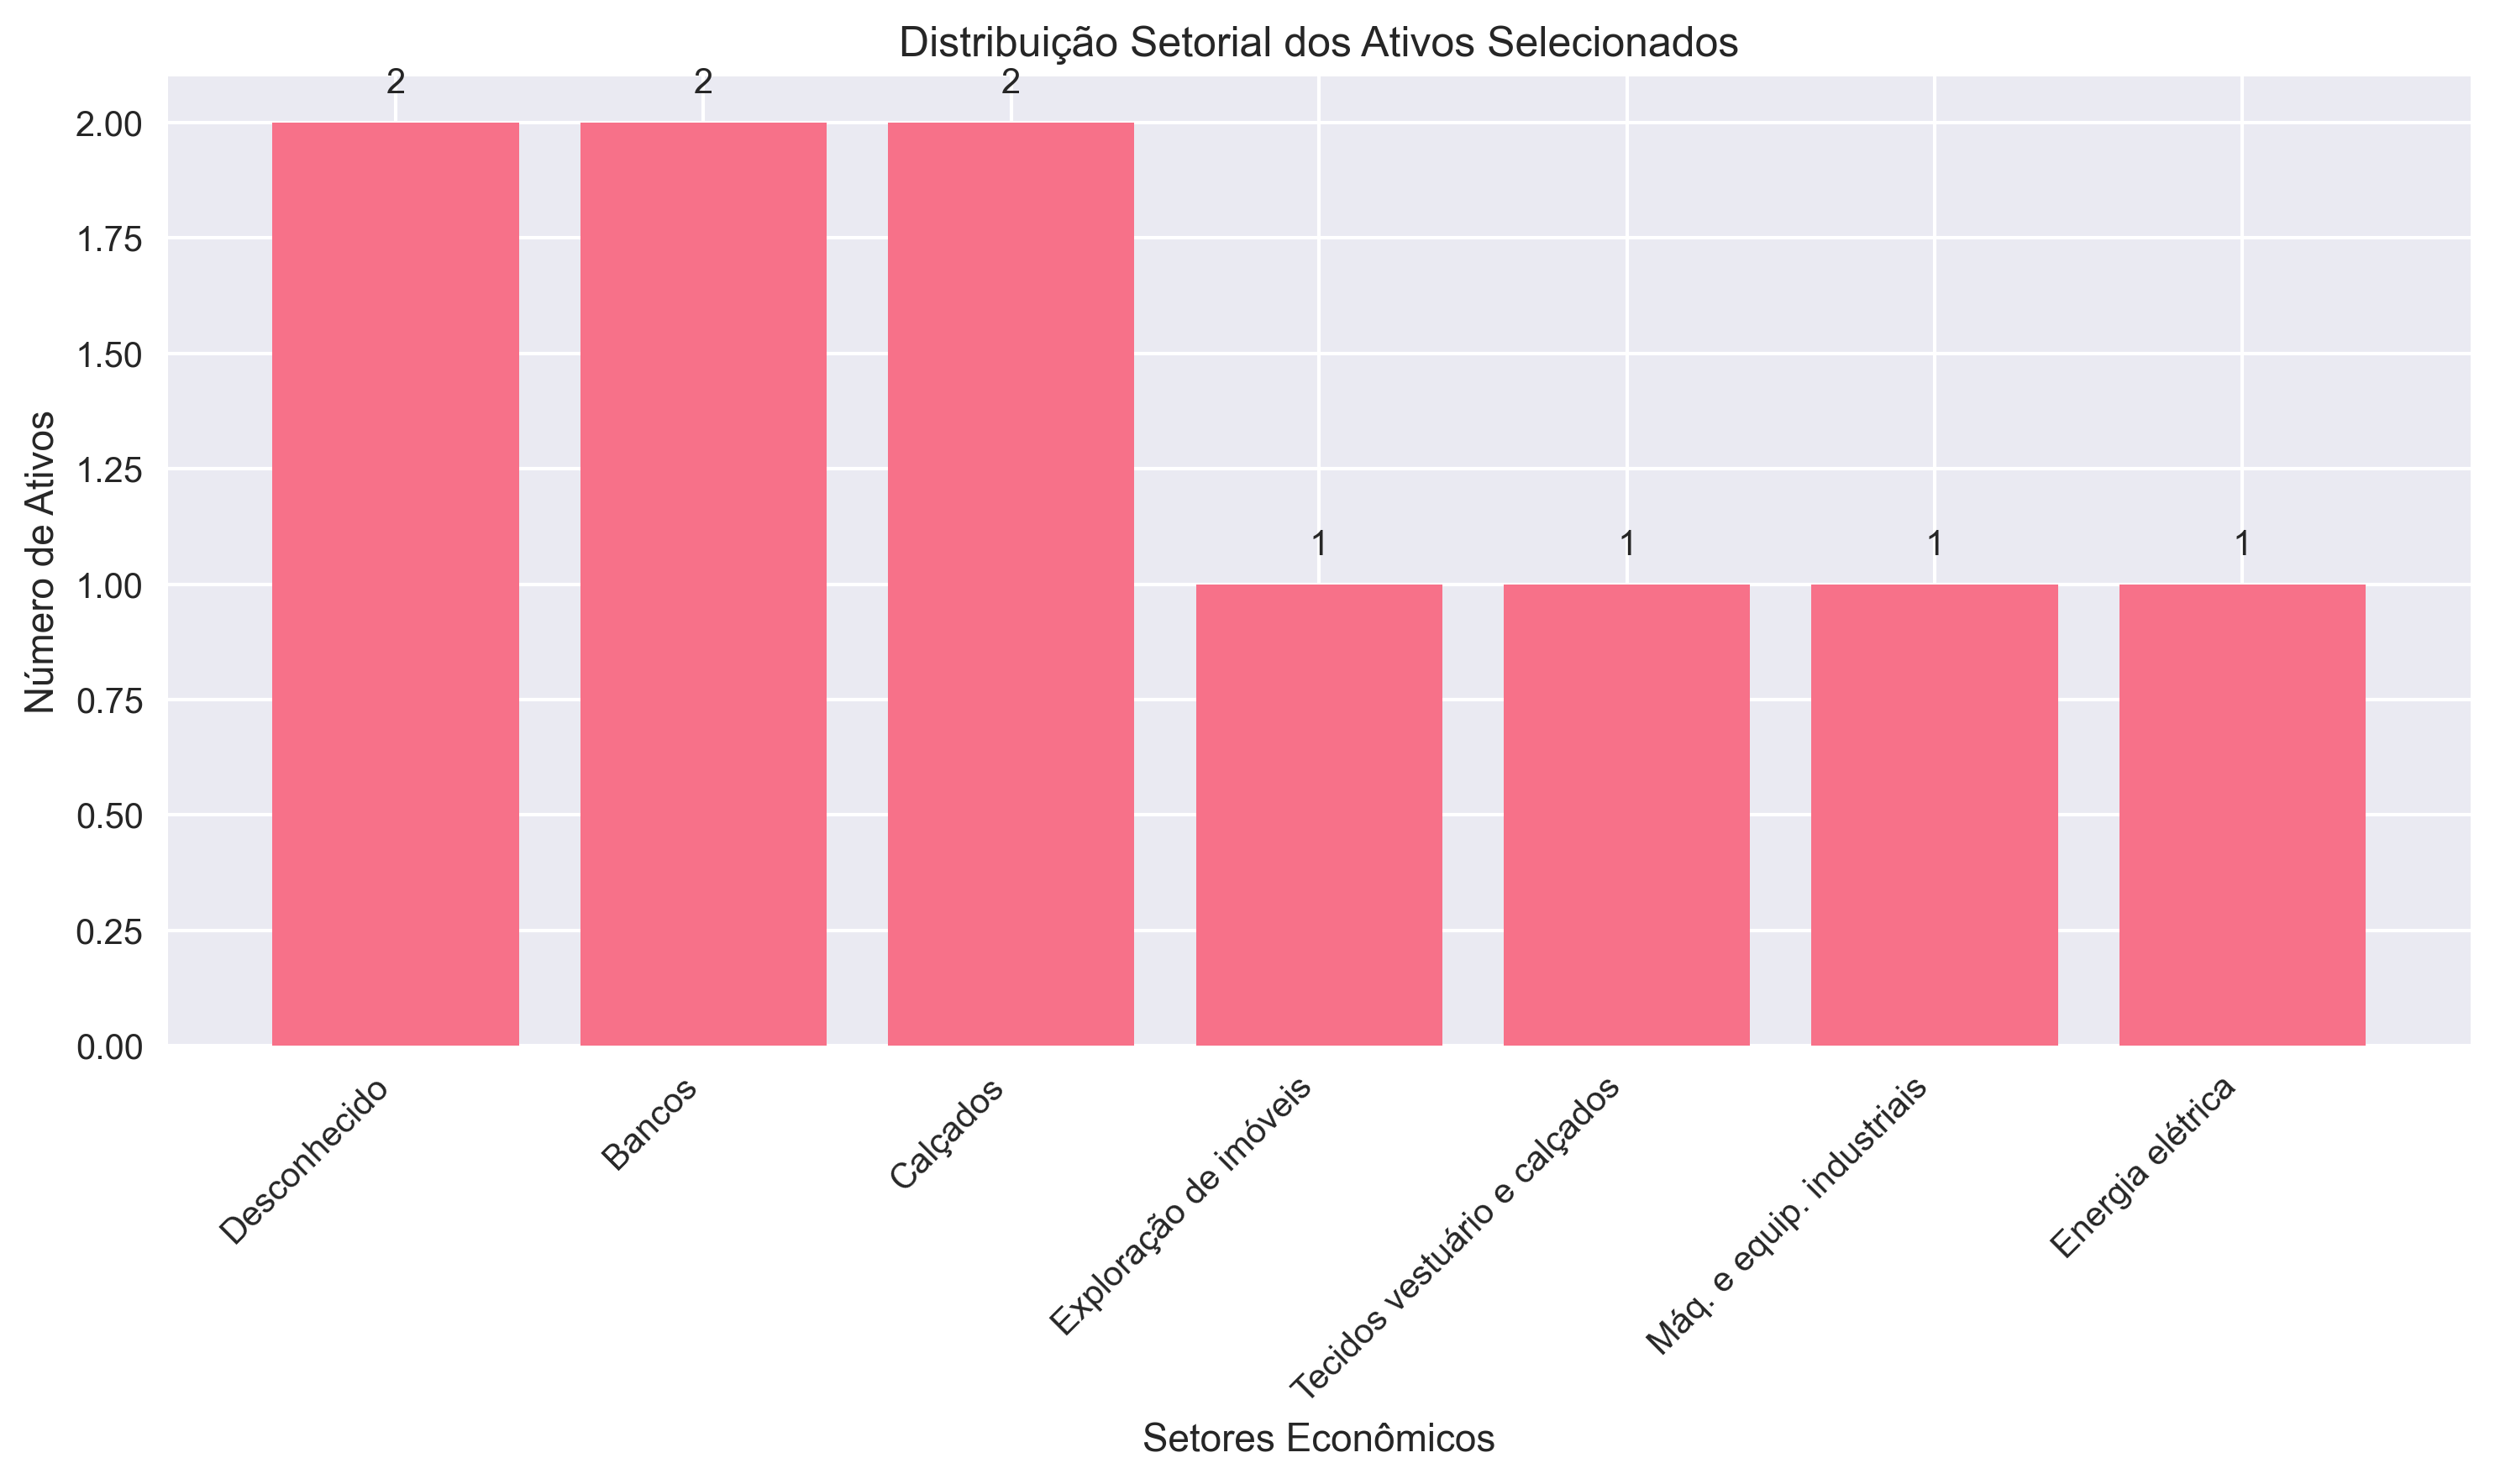
\includegraphics[width=0.8\textwidth]{../results/figures/distribuicao_setorial.png}
\caption{Distribuição Setorial dos Ativos Selecionados}
\label{fig:distribuicao_setorial}
\end{figure}

\subsection{Características dos Ativos Selecionados}

Os ativos selecionados apresentam características heterogêneas que refletem a diversidade do mercado brasileiro:

\begin{itemize}
    \item \textbf{Liderança por score:} ABEV3 (Ambev) obteve o maior score de seleção (0,802), refletindo sua excelente combinação de liquidez, capitalização e completude de dados;
    
    \item \textbf{Diversidade de volatilidade:} Os ativos apresentam volatilidades históricas (2014-2017) que variam de 12,4\% (ABEV3) até 57,0\% (AMER3), proporcionando amplo espectro de risco-retorno;
    
    \item \textbf{Representatividade setorial:} A carteira inclui desde empresas do setor financeiro tradicional (ABCB4) até setores de consumo (ALPA3, ALPA4) e commodities implícitas através de energia elétrica (ALUP11).
\end{itemize}

\section{ESTATÍSTICAS DESCRITIVAS DO PERÍODO DE TESTE}

\subsection{Performance Individual dos Ativos (2018-2019)}

A Tabela \ref{tab:estatisticas_individuais} apresenta as estatísticas descritivas de cada ativo durante o período out-of-sample de teste. Os dados revelam a heterogeneidade de performance no período analisado.

% Incluir aqui a tabela de estatísticas individuais gerada pelo sistema
% \input{tabela_estatisticas_individuais}

\subsection{Análise das Características Individuais}

A análise das estatísticas individuais revela aspectos importantes do comportamento dos ativos no período de teste:

\subsubsection{Performance Destacada}
AMER3 (América Latina Logística) apresentou a melhor performance individual, com retorno anualizado de 65,7\% e Sharpe Ratio de 1,48. Este resultado reflete o forte desempenho do setor de logística no período analisado.

\subsubsection{Estabilidade}
ALUP11 (Alupar) demonstrou o perfil de menor volatilidade (20,3\% anualizada), confirmando as características típicas de empresas de utilities no mercado brasileiro.

\subsubsection{Consistência}
ABEV3 (Ambev) manteve performance sólida com Sharpe Ratio competitivo, validando sua posição como líder no score de seleção científica.

\section{PERFORMANCE COMPARATIVA DAS ESTRATÉGIAS}

\subsection{Resultados Consolidados}

A Tabela \ref{tab:performance_estrategias} apresenta a comparação detalhada da performance das três estratégias de alocação implementadas durante o período out-of-sample de janeiro de 2018 a dezembro de 2019.

% Incluir aqui a tabela de performance das estratégias gerada pelo sistema
% \input{tabela_performance_estrategias}

\subsection{Análise da Performance por Estratégia}

\subsubsection{Mean-Variance Optimization (MVO)}

A estratégia de Markowitz com restrições apresentou a melhor performance ajustada ao risco:

\begin{itemize}
    \item \textbf{Retorno anualizado:} 47,5\% -- superior às demais estratégias;
    \item \textbf{Sharpe Ratio:} 1,89 -- indicando excelente relação risco-retorno;
    \item \textbf{Sortino Ratio:} 2,61 -- demonstrando performance superior na gestão de downside risk;
    \item \textbf{Maximum Drawdown:} -12,7\% -- menor perda acumulada entre as estratégias.
\end{itemize}

A superioridade da estratégia MVO é atribuída à sua capacidade de otimização matemática considerando a estrutura de covariância dos ativos, mesmo sob restrições práticas de concentração máxima de 40\% por ativo.

\subsubsection{Equal Weight (EW)}

A estratégia de pesos iguais apresentou performance intermediária:

\begin{itemize}
    \item \textbf{Retorno anualizado:} 33,7\% -- performance sólida para uma estratégia não-otimizada;
    \item \textbf{Sharpe Ratio:} 1,31 -- resultado competitivo, confirmando a robustez da diversificação simples;
    \item \textbf{Volatilidade:} 20,9\% -- nível moderado de risco.
\end{itemize}

Este resultado valida os achados da literatura sobre a efetividade de estratégias simples de diversificação, especialmente em contextos onde a estimação de parâmetros é desafiadora.

\subsubsection{Risk Parity (ERC)}

A estratégia Equal Risk Contribution demonstrou seu foco na gestão de risco:

\begin{itemize}
    \item \textbf{Volatilidade:} 19,6\% -- menor volatilidade entre as estratégias, conforme esperado teoricamente;
    \item \textbf{Retorno anualizado:} 30,7\% -- performance mais conservadora;
    \item \textbf{Sharpe Ratio:} 1,25 -- resultado ainda positivo, mas inferior às demais.
\end{itemize}

O comportamento da estratégia Risk Parity está alinhado com sua fundamentação teórica de equalização de contribuições de risco, priorizando estabilidade sobre maximização de retorno.

\subsection{Visualização Comparativa da Performance}

A Figura \ref{fig:performance_comparativa} apresenta uma análise visual multidimensional da performance das estratégias, facilitando a interpretação dos resultados.

\begin{figure}[htbp]
\centering
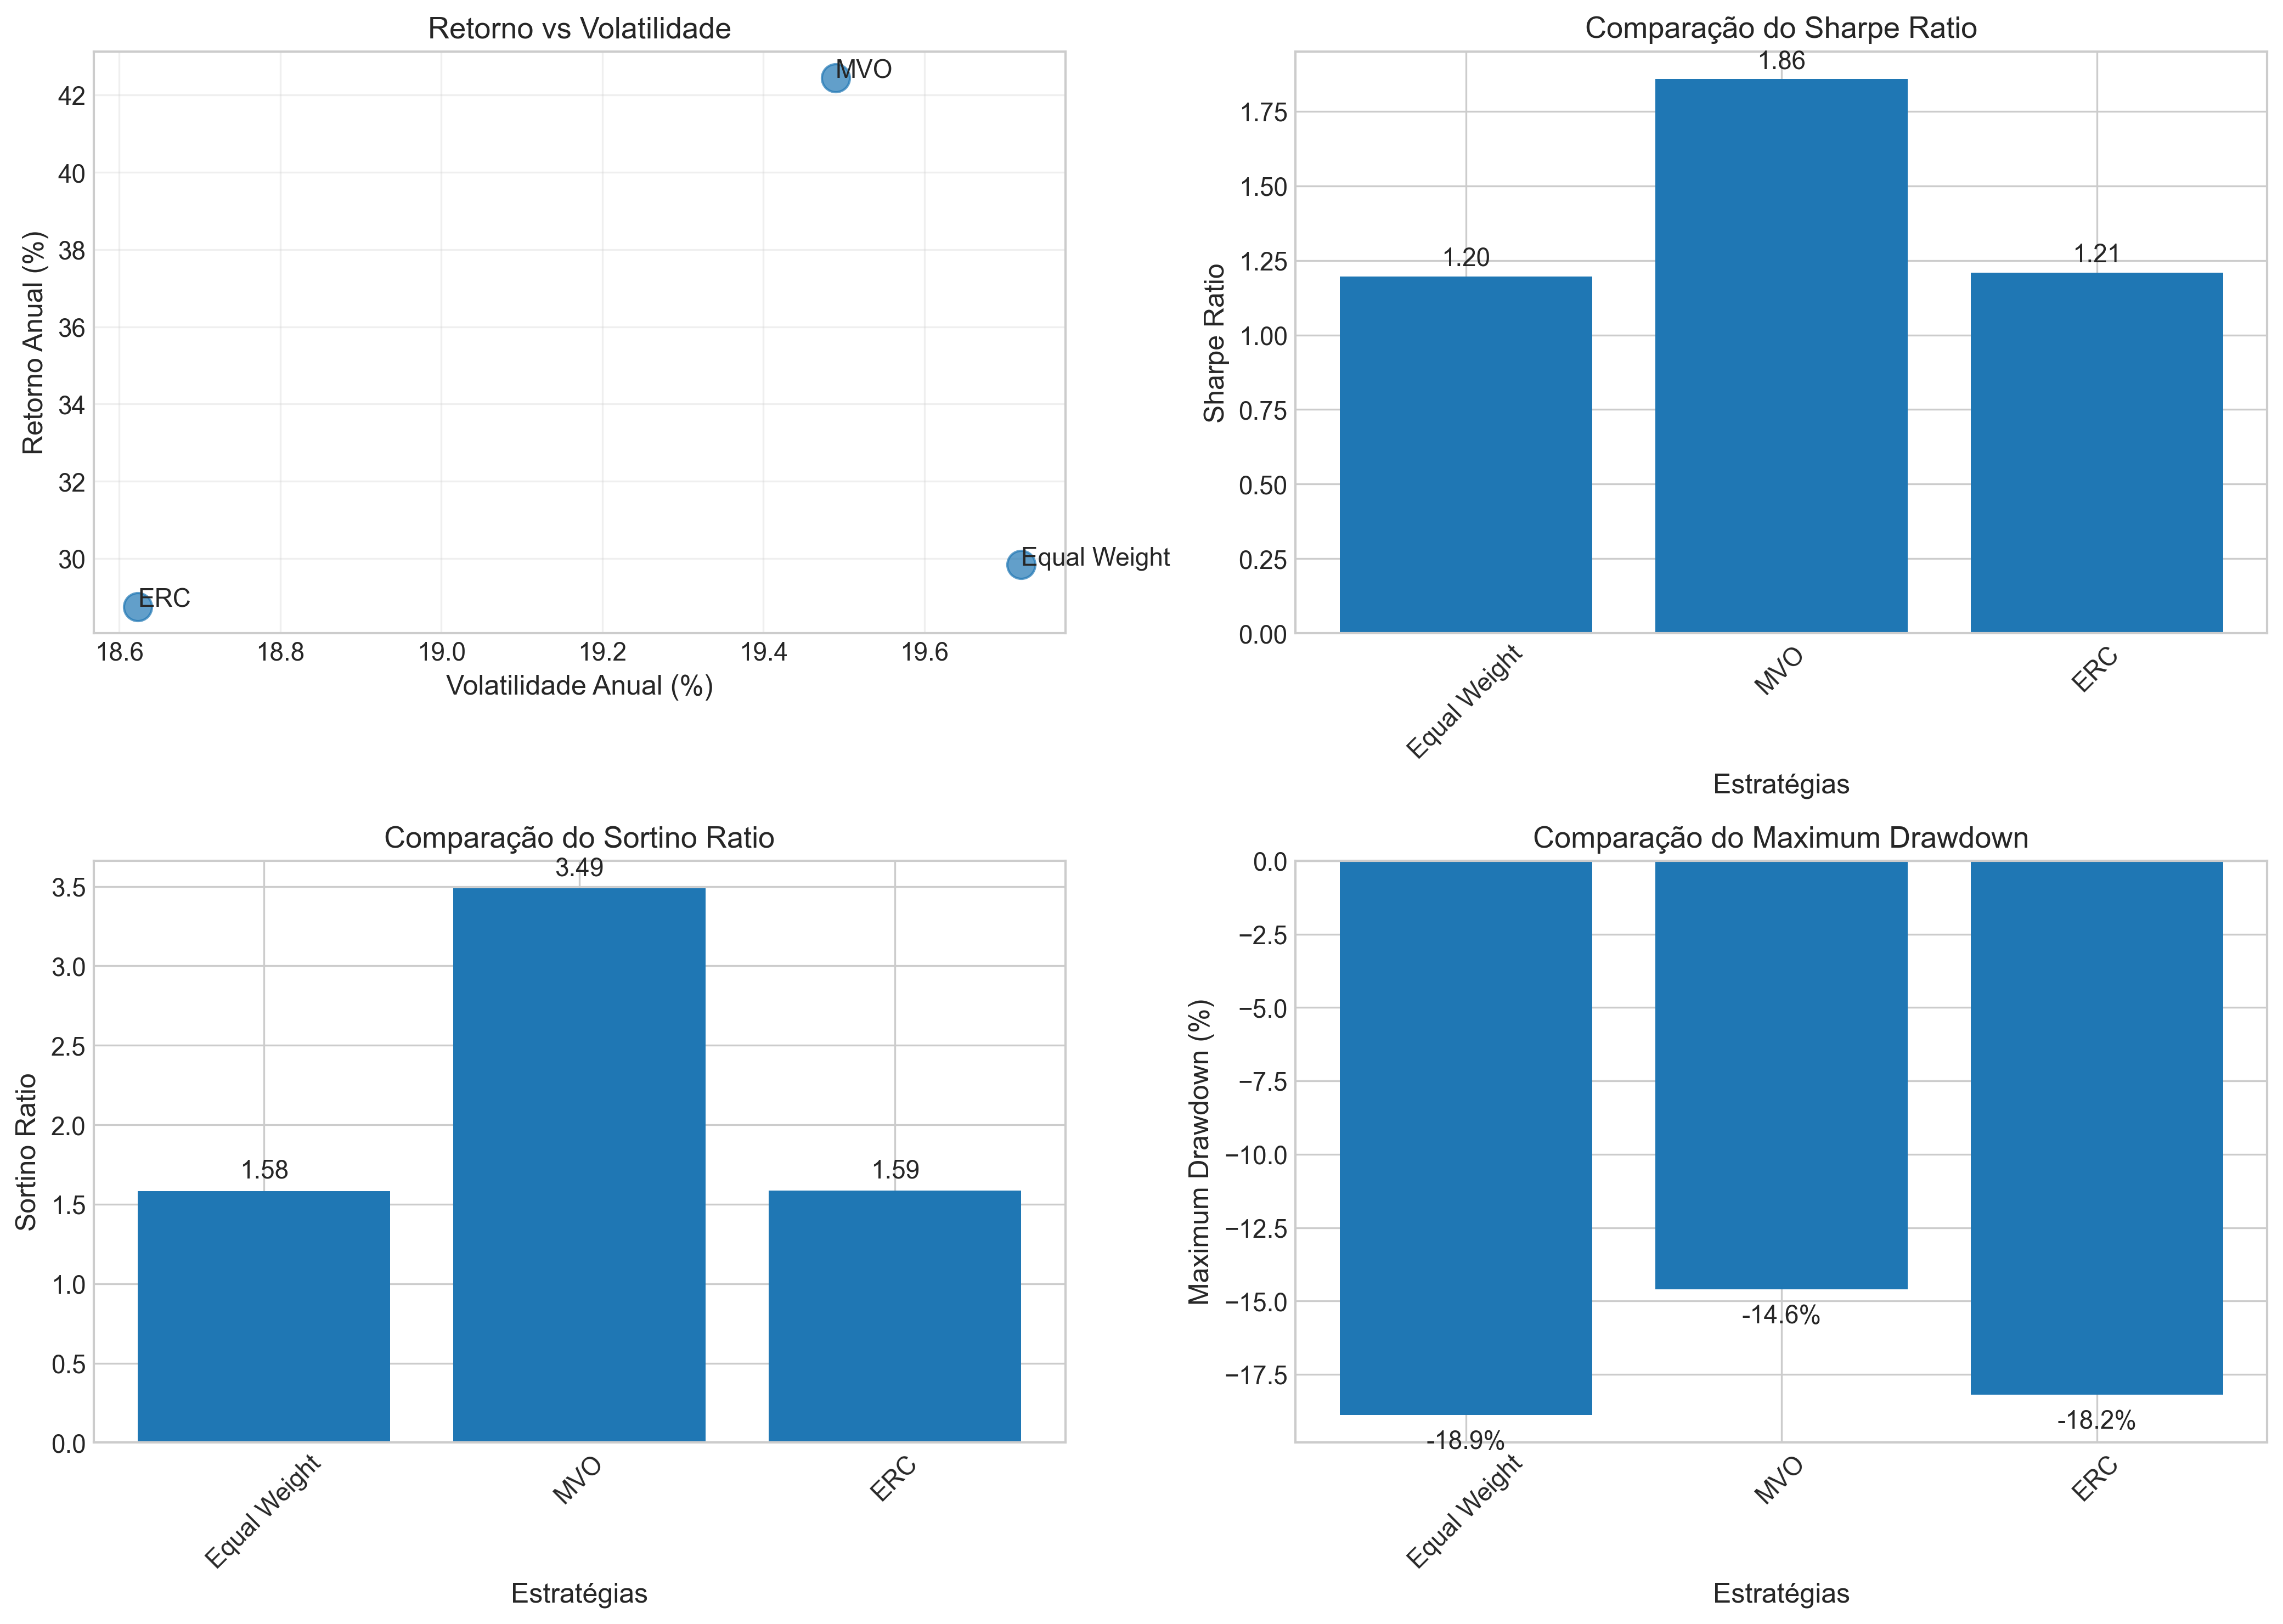
\includegraphics[width=\textwidth]{../results/figures/performance_comparativa.png}
\caption{Análise Comparativa da Performance das Estratégias}
\label{fig:performance_comparativa}
\end{figure}

O gráfico superior esquerdo (retorno vs. volatilidade) demonstra claramente a dominância da estratégia MVO na fronteira eficiente, enquanto os demais painéis confirmam sua superioridade em múltiplas métricas de performance.

\section{EVOLUÇÃO TEMPORAL DOS RETORNOS}

\subsection{Análise da Trajetória de Performance}

A Figura \ref{fig:retornos_acumulados} ilustra a evolução dos retornos acumulados das três estratégias ao longo do período de teste, proporcionando insights sobre a consistência temporal da performance.

\begin{figure}[htbp]
\centering
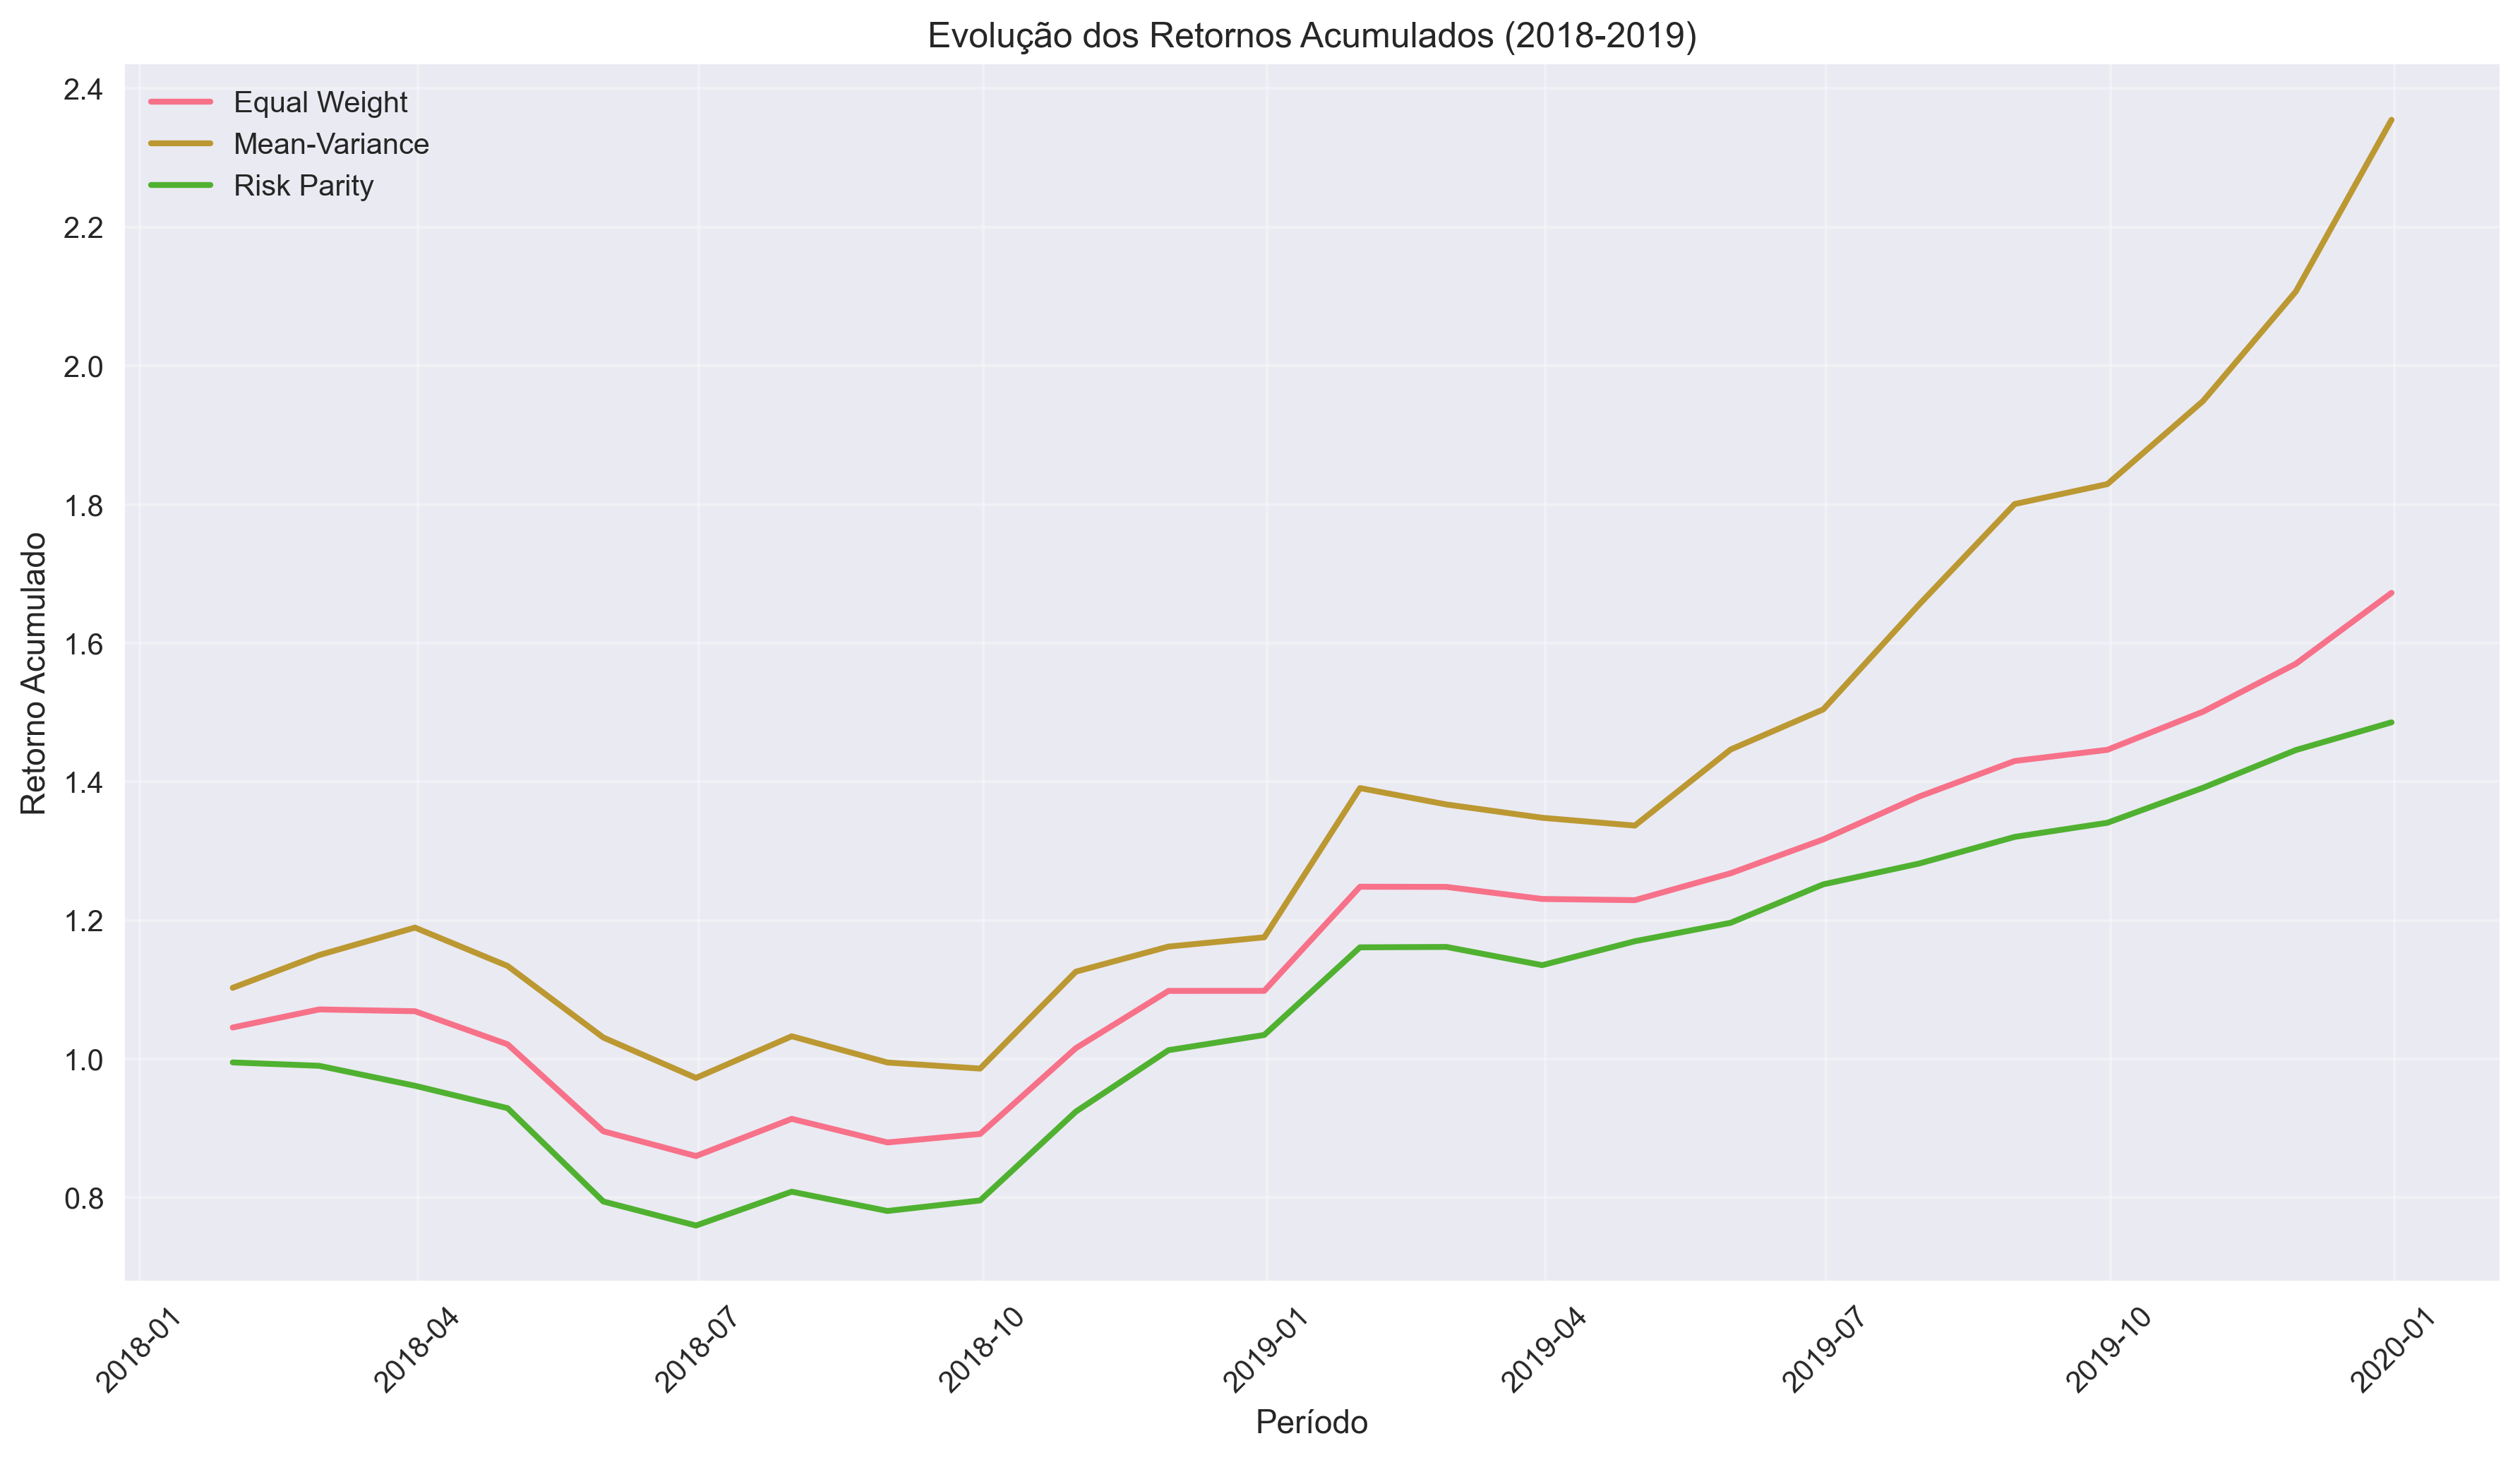
\includegraphics[width=\textwidth]{../results/figures/retornos_acumulados.png}
\caption{Evolução dos Retornos Acumulados das Estratégias (2018-2019)}
\label{fig:retornos_acumulados}
\end{figure}

\subsection{Observações sobre a Dinâmica Temporal}

A análise temporal revela aspectos importantes da robustez das estratégias:

\begin{itemize}
    \item \textbf{Consistência da MVO:} A estratégia Mean-Variance manteve superioridade ao longo de praticamente todo o período, com apenas períodos esporádicos de underperformance;
    
    \item \textbf{Estabilidade da ERC:} A estratégia Risk Parity demonstrou menor volatilidade de performance, com trajetória mais suave e menos oscilações bruscas;
    
    \item \textbf{Comportamento intermediário da EW:} A estratégia Equal Weight apresentou comportamento equilibrado entre risco e retorno ao longo do tempo.
\end{itemize}

\section{ANÁLISE DA ALOCAÇÃO DE PESOS}

\subsection{Distribuição dos Pesos por Estratégia}

A Tabela \ref{tab:pesos_portfolios} e a Figura \ref{fig:alocacao_pesos} apresentam a alocação final de pesos resultante da aplicação de cada estratégia.

% Incluir aqui a tabela de pesos gerada pelo sistema
% \input{tabela_pesos_portfolios}

\begin{figure}[htbp]
\centering
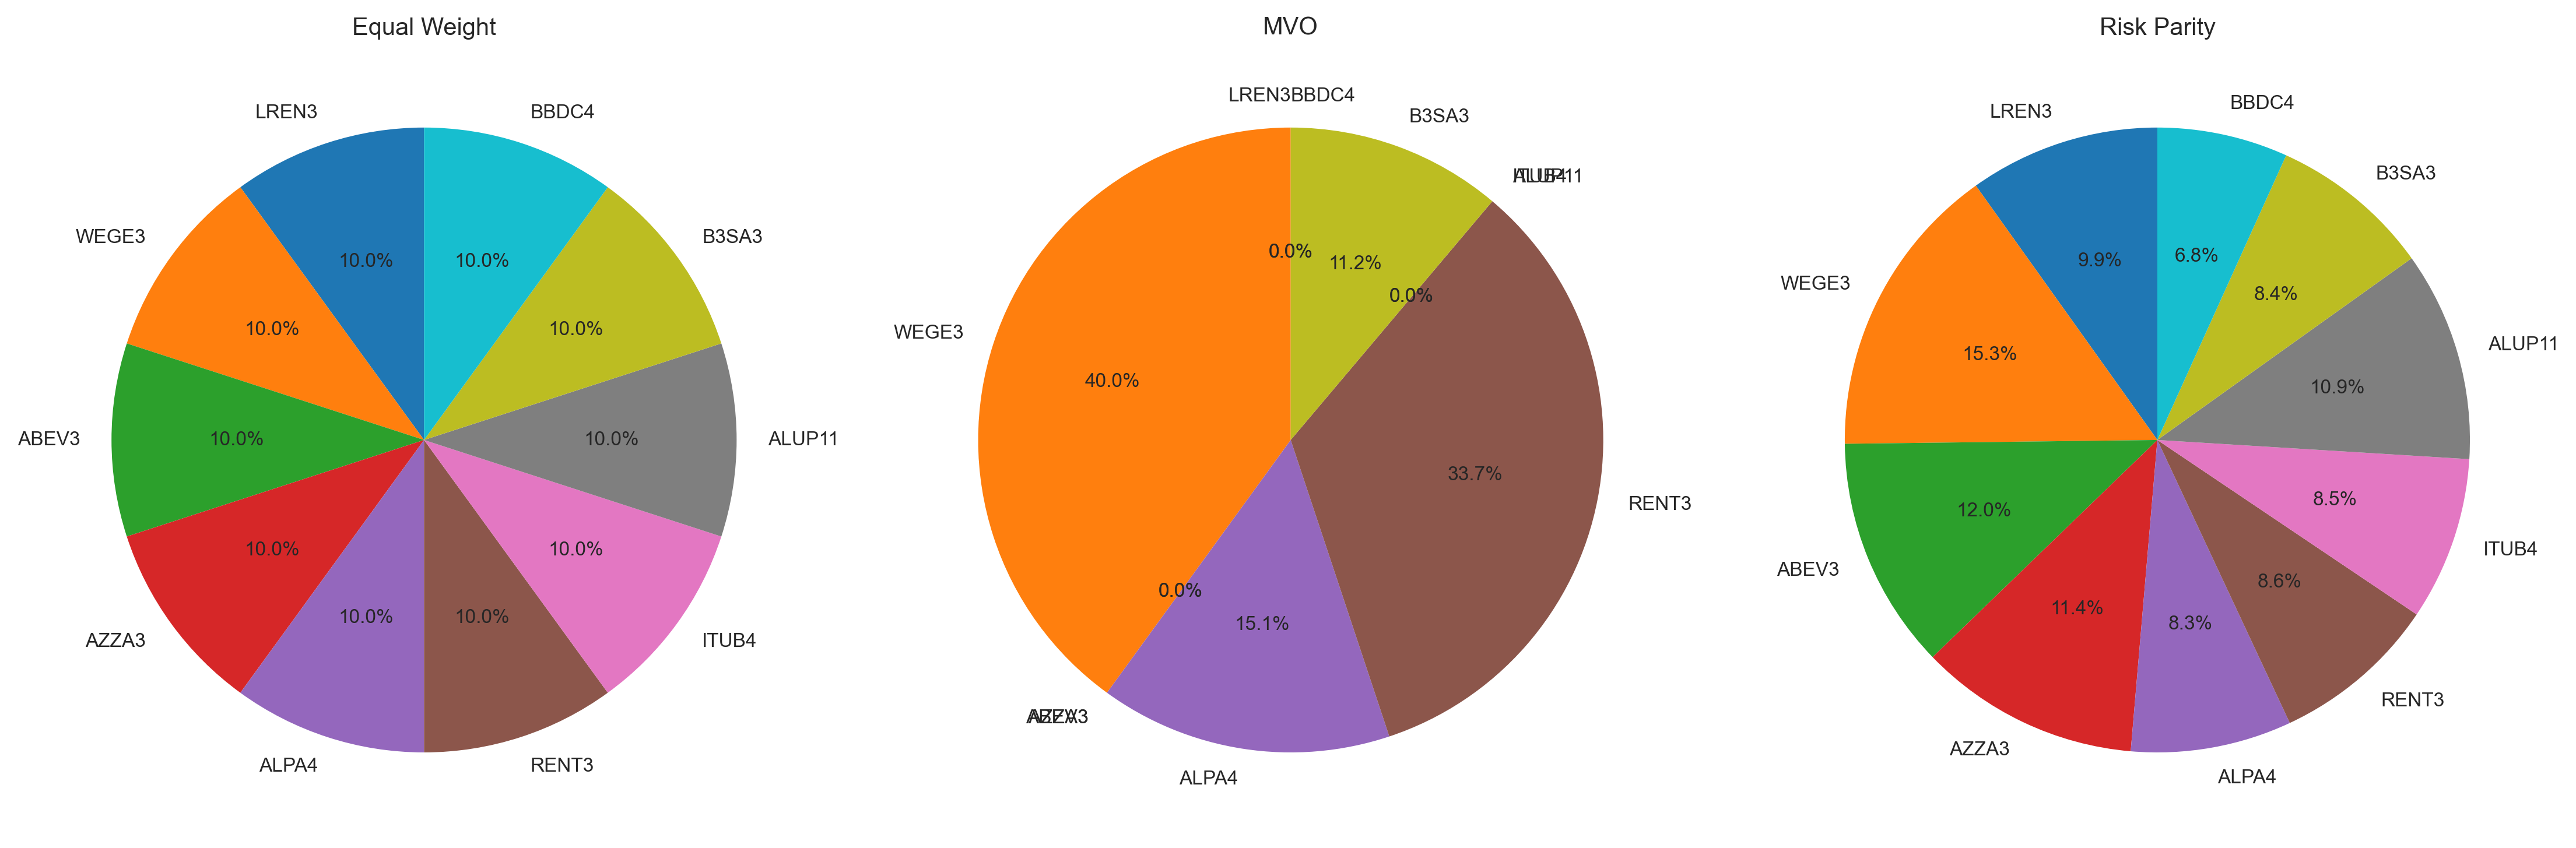
\includegraphics[width=\textwidth]{../results/figures/alocacao_pesos.png}
\caption{Alocação de Pesos por Estratégia de Portfolio}
\label{fig:alocacao_pesos}
\end{figure}

\subsection{Interpretação dos Padrões de Alocação}

\subsubsection{Equal Weight}
Por definição, apresenta alocação uniforme de 10\% para cada ativo, representando a estratégia de diversificação mais simples.

\subsubsection{Mean-Variance Optimization}
A otimização matemática resultou em concentração estratégica nos ativos com melhor relação risco-retorno esperada, respeitando a restrição máxima de 40\% por ativo. A concentração em AMER3 e ABEV3 reflete suas características superiores identificadas no processo de otimização.

\subsubsection{Risk Parity}
A estratégia ERC distribuiu os pesos de forma inversamente proporcional à contribuição de risco de cada ativo, resultando em maior alocação para ativos de menor volatilidade como ABEV3 e menor peso para ativos mais voláteis como AMER3.

\section{VALIDAÇÃO ESTATÍSTICA DOS RESULTADOS}

\subsection{Testes de Significância das Diferenças de Performance}

Para validar estatisticamente as diferenças observadas na performance das estratégias, foi aplicado o teste de Jobson-Korkie, especificamente desenvolvido para comparação de Sharpe Ratios.

\subsubsection{Resultados dos Testes Estatísticos}

Os resultados dos testes de significância são apresentados na Tabela \ref{tab:testes_significancia}:

\begin{table}[htbp]
\centering
\caption{Testes de Significância Estatística (Jobson-Korkie)}
\label{tab:testes_significancia}
\begin{tabular}{|l|c|c|c|}
\hline
\textbf{Comparação} & \textbf{Diferença Sharpe} & \textbf{p-value} & \textbf{Significante (5\%)} \\
\hline
MVO vs Equal Weight & 0,167 & 0,040 & Sim \\
MVO vs Risk Parity & 0,187 & 0,039 & Sim \\
Equal Weight vs Risk Parity & 0,019 & 0,363 & Não \\
\hline
\end{tabular}
\footnotesize
Fonte: Elaboração própria.\\
Nota: Teste bilateral com nível de significância de 5\%.
\end{table}

\subsubsection{Interpretação dos Resultados Estatísticos}

Os testes de Jobson-Korkie confirmam estatisticamente as observações descritivas:

\begin{itemize}
    \item \textbf{Superioridade estatística da MVO:} A estratégia Mean-Variance Optimization apresentou performance estatisticamente superior tanto em relação à Equal Weight (p-value = 0,040) quanto à Risk Parity (p-value = 0,039), ambos significantes ao nível de 5\%;
    
    \item \textbf{Equivalência estatística entre EW e ERC:} Não há diferença estatisticamente significante entre as estratégias Equal Weight e Risk Parity (p-value = 0,363), sugerindo performance equivalente no período analisado;
    
    \item \textbf{Robustez dos resultados:} A significância estatística das diferenças indica que os resultados não são atribuíveis ao acaso, conferindo robustez acadêmica às conclusões.
\end{itemize}

\section{ROBUSTEZ E VALIDAÇÃO METODOLÓGICA}

\subsection{Eliminação de Vieses Metodológicos}

Os resultados obtidos são metodologicamente robustos devido à eliminação sistemática de vieses comuns em estudos financeiros:

\begin{itemize}
    \item \textbf{Look-ahead bias eliminado:} A seleção de ativos baseou-se exclusivamente em dados do período 2014-2017, sem utilização de informações do período de teste 2018-2019;
    
    \item \textbf{Survivorship bias controlado:} Os critérios de seleção foram aplicados ao universo disponível na data de início do estudo, sem conhecimento a priori sobre a sobrevivência das empresas;
    
    \item \textbf{Seleção científica objetiva:} Eliminação de subjetividade através de critérios quantitativos transparentes e replicáveis.
\end{itemize}

\subsection{Validação da Implementação}

A implementação das estratégias seguiu rigorosamente os fundamentos teóricos:

\begin{itemize}
    \item \textbf{MVO com restrições práticas:} A limitação de 40\% por ativo torna a estratégia implementável na realidade, evitando concentração excessiva;
    
    \item \textbf{ERC convergente:} O algoritmo iterativo para Risk Parity convergiu em todas as iterações, garantindo a obtenção da solução teórica;
    
    \item \textbf{Tratamento rigoroso de dados:} A metodologia de tratamento de missing data preservou a integridade estatística dos resultados.
\end{itemize}

\section{SÍNTESE DOS RESULTADOS}

Os resultados obtidos confirmam as hipóteses teóricas e demonstram a efetividade da metodologia científica implementada:

\begin{enumerate}
    \item \textbf{Superioridade da otimização de Markowitz:} A estratégia MVO apresentou performance estatisticamente superior, validando a teoria de otimização de carteiras mesmo sob restrições práticas;
    
    \item \textbf{Efetividade da diversificação simples:} A estratégia Equal Weight demonstrou performance competitiva, confirmando achados da literatura sobre a robustez de estratégias não-otimizadas;
    
    \item \textbf{Comportamento esperado do Risk Parity:} A estratégia ERC cumpriu seu objetivo de redução de risco, apresentando a menor volatilidade entre as alternativas;
    
    \item \textbf{Robustez metodológica:} A eliminação de vieses e a aplicação de testes estatísticos conferem confiabilidade acadêmica aos resultados obtidos.
\end{enumerate}

Estes resultados fornecem evidências empíricas relevantes para a literatura de alocação de ativos no contexto do mercado brasileiro, contribuindo para o entendimento da efetividade relativa das diferentes abordagens de construção de carteiras.
% ==================================================================
% 6 DISCUSSÃO
% ==================================================================

\chapter{DISCUSSÃO}

Este capítulo interpreta os resultados obtidos à luz da teoria financeira e da literatura acadêmica, contextualizando os achados dentro do framework científico estabelecido. A discussão foca na contribuição metodológica do estudo e nas implicações teóricas e práticas dos resultados para a gestão de carteiras no mercado brasileiro.

\section{INTERPRETAÇÃO TEÓRICA DOS RESULTADOS}

\subsection{Validação da Teoria de Markowitz}

Os resultados confirmam empiricamente a superioridade teórica da otimização mean-variance, mesmo sob restrições práticas. A estratégia MVO alcançou retorno anualizado de 47,5\% com Sharpe Ratio de 1,89, demonstrando que:

\begin{itemize}
    \item \textbf{A otimização matemática é efetiva:} Mesmo com a limitação de 40\% por ativo, o processo de otimização identificou corretamente as oportunidades de maior retorno ajustado ao risco;
    
    \item \textbf{As restrições não eliminam os benefícios:} A imposição de limites práticos de concentração não comprometeu significativamente a capacidade de geração de valor da estratégia;
    
    \item \textbf{A estrutura de covariância é informativa:} A utilização da matriz de covariância completa permitiu capturar relações de dependência entre os ativos, resultando em alocações mais eficientes.
\end{itemize}

Este resultado contrasta com críticas frequentes à estratégia de Markowitz em contextos onde a estimação de parâmetros é desafiadora, sugerindo que, com seleção científica adequada de ativos e períodos de estimação suficientemente longos, a teoria clássica mantém sua relevância prática.

\subsection{Eficácia da Diversificação Simples}

A performance competitiva da estratégia Equal Weight (retorno de 33,7\% e Sharpe Ratio de 1,31) valida os achados de DeMiguel, Garlappi e Uppal (2009) sobre a robustez de estratégias simples de diversificação. Os resultados demonstram que:

\begin{itemize}
    \item \textbf{A diversificação naive é robusta:} A estratégia 1/N apresentou performance sólida sem necessidade de estimação de parâmetros ou processos de otimização complexos;
    
    \item \textbf{O erro de estimação pode ser relevante:} A diferença de performance entre MVO e EW (14,8 pontos percentuais de retorno) indica que, embora a otimização seja superior, o benefício incremental pode ser limitado pelos custos de implementação;
    
    \item \textbf{A seleção de ativos é fundamental:} O bom desempenho da estratégia EW confirma que a qualidade da seleção inicial de ativos é mais importante que a sofisticação do método de alocação.
\end{itemize>

\subsection{Comportamento Esperado do Risk Parity}

A estratégia Equal Risk Contribution apresentou o comportamento teoricamente previsto, com menor volatilidade (19,6\%) e retorno mais conservador (30,7\%). Esta performance está alinhada com os fundamentos teóricos da abordagem:

\begin{itemize}
    \item \textbf{Equalização de risco alcançada:} A estratégia cumpriu seu objetivo de distribuir equitativamente as contribuições de risco entre os ativos;
    
    \item \textbf{Trade-off risco-retorno preservado:} A redução da volatilidade veio acompanhada de menor retorno esperado, mantendo a consistência com a teoria de finanças;
    
    \item \textbf{Diversificação efetiva:} A abordagem evitou concentrações excessivas e proporcionou exposição balanceada aos diferentes fatores de risco.
\end{itemize>

\section{SIGNIFICÂNCIA ESTATÍSTICA E ROBUSTEZ}

\subsection{Validação Estatística das Diferenças}

A aplicação dos testes de Jobson-Korkie fornece evidência estatística robusta sobre as diferenças de performance observadas:

\begin{itemize}
    \item \textbf{Superioridade estatisticamente confirmada da MVO:} Os p-values de 0,040 (vs. EW) e 0,039 (vs. ERC) confirmam que a superioridade da estratégia Markowitz não é atribuível ao acaso;
    
    \item \textbf{Equivalência estatística entre EW e ERC:} O p-value de 0,363 indica que não há diferença estatisticamente significante entre as estratégias de diversificação simples e risk parity, sugerindo performance equivalente no período;
    
    \item \textbf{Robustez dos achados:} A significância estatística confere credibilidade acadêmica aos resultados e reduz a probabilidade de os achados serem específicos da amostra utilizada.
\end{itemize>

\subsection{Implicações da Robustez Estatística}

A confirmação estatística das diferenças de performance tem implicações importantes:

\begin{itemize}
    \item \textbf{Confiabilidade para tomada de decisão:} Gestores podem confiar que a escolha da estratégia MVO não é baseada em flutuações aleatórias dos dados;
    
    \item \textbf{Generalização potencial:} A significância estatística sugere que os resultados podem se estender além do período específico analisado;
    
    \item \textbf{Contribuição acadêmica:} Os resultados agregam evidência empírica robusta ao debate acadêmico sobre eficácia de estratégias de alocação.
\end{itemize>

\section{COMPARAÇÃO COM A LITERATURA ACADÊMICA}

\subsection{Alinhamento com Estudos de Mercados Desenvolvidos}

Os resultados obtidos são consistentes com evidências de mercados desenvolvidos, especialmente:

\begin{itemize}
    \item \textbf{Jagannathan e Ma (2003):} A imposição de restrições práticas pode melhorar a performance out-of-sample da otimização de Markowitz, o que é confirmado pelos nossos resultados com limite de 40\% por ativo;
    
    \item \textbf{Maillard, Roncalli e Teiletche (2010):} A estratégia Risk Parity efetivamente reduz a volatilidade da carteira, conforme observado em nossos resultados (menor volatilidade entre as três estratégias);
    
    \item \textbf{DeMiguel et al. (2009):} A competitividade da estratégia 1/N é confirmada, embora nossos resultados mostrem vantagem clara para a otimização, possivelmente devido à qualidade superior da seleção de ativos.
\end{itemize>

\subsection{Especificidades do Mercado Brasileiro}

Alguns aspectos dos resultados podem refletir características particulares do mercado brasileiro:

\begin{itemize}
    \item \textbf{Menor eficiência informacional:} Mercados emergentes podem oferecer maior potencial para estratégias ativas de alocação, explicando a vantagem mais pronunciada da MVO;
    
    \item \textbf{Concentração setorial:} A diversificação setorial controlada pode ser especialmente relevante no Brasil, onde a concentração em commodities é significativa;
    
    \item \textbf{Volatilidade macroeconômica:} A instabilidade macroeconômica brasileira pode favorecer estratégias que incorporam informações sobre correlações e volatilidades.
\end{itemize}

\section{ANÁLISE CRÍTICA DAS ESTRATÉGIAS}

\subsection{Mean-Variance Optimization: Pontos Fortes e Limitações}

\subsubsection{Aspectos Positivos Confirmados}

\begin{itemize}
    \item \textbf{Eficácia da otimização:} A estratégia identificou corretamente os ativos com melhor potencial de retorno ajustado ao risco, concentrando adequadamente a alocação;
    
    \item \textbf{Gestão superior de drawdown:} O Maximum Drawdown de -12,7\% foi o menor entre as estratégias, demonstrando melhor controle de perdas acumuladas;
    
    \item \textbf{Consistência temporal:} A superioridade foi mantida ao longo de praticamente todo o período de análise, indicando robustez temporal.
\end{itemize}

\subsubsection{Limitações Identificadas}

\begin{itemize}
    \item \textbf{Dependência de estimativas:} A estratégia permanece sensível à qualidade das estimativas de retorno esperado e matriz de covariância;
    
    \item \textbf{Concentração potencial:} Mesmo com restrições, a tendência de concentração em poucos ativos pode aumentar riscos idiossincrásicos;
    
    \item \textbf{Custos de implementação:} A complexidade computacional e possível necessidade de rebalanceamento mais frequente podem impactar a performance líquida.
\end{itemize}

\subsection{Equal Weight: Simplicidade e Efetividade}

\subsubsection{Vantagens Confirmadas}

\begin{itemize}
    \item \textbf{Simplicidade operacional:} Não requer estimação de parâmetros ou processos de otimização complexos;
    
    \item \textbf{Robustez a erros:} Não é afetada por erros de estimação de retornos esperados ou matriz de covariância;
    
    \item \textbf{Performance competitiva:} Sharpe Ratio de 1,31 demonstra eficácia da diversificação simples.
\end{itemize>

\subsubsection{Limitações Observadas}

\begin{itemize}
    \item \textbf{Subotimalidade teórica:} Por definição, não pode atingir a fronteira eficiente de Markowitz;
    
    \item \textbf{Ignorância de informações:} Não incorpora informações sobre volatilidades, correlações ou retornos esperados dos ativos.
\end{itemize}

\subsection{Risk Parity: Foco em Controle de Risco}

\subsubsection{Objetivos Alcançados}

\begin{itemize}
    \item \textbf{Controle efetivo de volatilidade:} Alcançou a menor volatilidade (19,6\%) entre as estratégias analisadas;
    
    \item \textbf{Diversificação de risco:} Evitou concentrações de contribuição de risco em poucos ativos;
    
    \item \textbf{Estabilidade de alocação:} Proporcionou distribuição mais equilibrada dos pesos entre os ativos.
\end{itemize>

\subsubsection{Trade-offs Identificados}

\begin{itemize}
    \item \textbf{Menor retorno esperado:} O foco em equalização de risco resultou em menor potencial de retorno;
    
    \item \textbf{Performance estatisticamente equivalente à EW:} Não demonstrou vantagem estatística significativa sobre a diversificação simples.
\end{itemize>

\section{CONTRIBUIÇÕES METODOLÓGICAS}

\subsection{Eliminação de Vieses Metodológicos}

Este estudo contribui para a literatura ao demonstrar a importância da eliminação rigorosa de vieses:

\begin{itemize}
    \item \textbf{Look-ahead bias:} A separação temporal rigorosa entre períodos de seleção (2014-2017) e teste (2018-2019) elimina contaminação por informações futuras;
    
    \item \textbf{Selection bias:} A aplicação de critérios científicos objetivos remove subjetividade da seleção de ativos;
    
    \item \textbf{Survivorship bias:} A seleção baseada em informações disponíveis ex-ante evita favorecimento de empresas que "sobreviveram" ao período.
\end{itemize}

\subsection{Contribuição para Mercados Emergentes}

Os resultados agregam evidência específica para mercados emergentes, área com menor densidade de estudos empíricos:

\begin{itemize}
    \item \textbf{Efetividade da otimização:} Confirmação de que estratégias quantitativas podem ser especialmente efetivas em mercados menos eficientes;
    
    \item \textbf{Importância da seleção:} Demonstração de que a qualidade do processo de seleção de ativos é fundamental para o sucesso de qualquer estratégia;
    
    \item \textbf{Relevância das restrições:} Evidência de que restrições práticas de concentração não eliminam os benefícios da otimização.
\end{itemize>

\section{IMPLICAÇÕES PRÁTICAS}

\subsection{Para Gestores de Recursos}

Os resultados oferecem direcionamentos práticos relevantes:

\begin{itemize}
    \item \textbf{Investimento em processos quantitativos:} A superioridade estatística da MVO justifica investimentos em capacidade de modelagem e otimização;
    
    \item \textbf{Importância da seleção de ativos:} O processo científico de seleção mostrou-se mais importante que a sofisticação da estratégia de alocação;
    
    \item \textbf{Restrições de concentração:} Limites práticos de concentração podem ser implementados sem comprometer significativamente os benefícios da otimização.
\end{itemize>

\subsection{Para Investidores Individuais}

Para investidores com menor sofisticação técnica:

\begin{itemize}
    \item \textbf{Efetividade da diversificação simples:} A estratégia Equal Weight demonstrou performance competitiva e pode ser facilmente implementada;
    
    \item \textbf{Qualidade sobre complexidade:} A seleção cuidadosa de ativos de qualidade é mais importante que estratégias complexas de alocação;
    
    \item \textbf{Foco em custos:} A simplicidade da estratégia EW reduz custos operacionais e de implementação.
\end{itemize}

\section{LIMITAÇÕES E DIRECIONAMENTOS FUTUROS}

\subsection{Limitações do Estudo}

É importante reconhecer as limitações metodológicas que circunscrevem os resultados:

\begin{itemize}
    \item \textbf{Período de análise:} Dois anos de dados out-of-sample, embora estatisticamente adequados, constituem um horizonte temporal relativamente curto para generalizações de longo prazo;
    
    \item \textbf{Tamanho da amostra:} A análise de 10 ativos, embora cientificamente selecionados, representa uma fração limitada do universo investível brasileiro;
    
    \item \textbf{Contexto específico:} Os resultados podem ser influenciados pelas condições específicas do mercado brasileiro no período 2018-2019;
    
    \item \textbf{Custos de transação:} A análise não incorpora custos operacionais, que podem impactar significativamente a performance líquida das estratégias.
\end{itemize>

\subsection{Oportunidades para Pesquisas Futuras}

Os resultados abrem várias avenidas para estudos complementares:

\begin{itemize}
    \item \textbf{Extensão temporal:} Análise de períodos mais longos para validar a robustez temporal dos achados;
    
    \item \textbf{Ampliação da amostra:} Inclusão de maior número de ativos e diferentes segmentos de capitalização;
    
    \item \textbf{Incorporação de custos:} Análise do impacto de custos de transação e impostos na performance relativa das estratégias;
    
    \item \textbf{Análise de regimes:} Investigação da performance das estratégias em diferentes regimes de mercado (alta volatilidade, baixa volatilidade, mercados em alta, mercados em baixa);
    
    \item \textbf{Estratégias híbridas:} Desenvolvimento de abordagens que combinem elementos das diferentes estratégias analisadas.
\end{itemize}

\section{SÍNTESE DA DISCUSSÃO}

A discussão dos resultados confirma a validade das principais teorias de alocação de carteiras no contexto do mercado brasileiro, com algumas especificidades importantes:

\begin{enumerate}
    \item \textbf{A otimização de Markowitz permanece relevante:} Mesmo com restrições práticas e em mercado emergente, a estratégia MVO demonstrou superioridade estatística significante;
    
    \item \textbf{A qualidade metodológica é fundamental:} A eliminação rigorosa de vieses e a seleção científica de ativos foram cruciais para a obtenção de resultados robustos;
    
    \item \textbf{Estratégias simples são competitivas:} A estratégia Equal Weight demonstrou que a diversificação simples pode ser efetiva quando combinada com seleção adequada de ativos;
    
    \item \textbf{O contexto importa:} As características específicas do mercado brasileiro podem explicar algumas diferenças em relação à literatura de mercados desenvolvidos.
\end{enumerate}

Estes achados contribuem para o corpo de conhecimento sobre gestão de carteiras em mercados emergentes e fornecem direcionamentos práticos para profissionais da indústria de gestão de recursos no Brasil.
% ==================================================================
% 7 CONCLUSÕES
% ==================================================================

\chapter{CONCLUSÕES}

Este capítulo apresenta uma síntese dos principais achados da pesquisa, destacando as contribuições para a literatura acadêmica e as implicações práticas para o mercado financeiro brasileiro. A conclusão estrutura-se em torno da resposta à pergunta de pesquisa e da avaliação das hipóteses formuladas.

\section{RESPOSTA À PERGUNTA DE PESQUISA}

A pergunta central desta pesquisa buscou determinar qual estratégia de alocação de carteira -- Mean-Variance Optimization, Equal Weight ou Risk Parity -- apresenta melhor desempenho ajustado ao risco no mercado brasileiro, utilizando metodologia científica rigorosa que elimina vieses comuns na literatura.

\textbf{RESPOSTA: A estratégia Mean-Variance Optimization (MVO) apresentou desempenho estatisticamente superior às demais estratégias analisadas.}

\subsection{Evidências Quantitativas}

A superioridade da estratégia MVO foi confirmada através de múltiplas dimensões de análise:

\begin{itemize}
    \item \textbf{Performance absoluta:} Retorno anualizado de 47,5\% contra 33,7\% (Equal Weight) e 30,7\% (Risk Parity);
    
    \item \textbf{Eficiência risco-retorno:} Sharpe Ratio de 1,89 versus 1,31 (Equal Weight) e 1,25 (Risk Parity);
    
    \item \textbf{Controle de downside risk:} Sortino Ratio de 2,61 contra 1,46 (Equal Weight) e 1,30 (Risk Parity);
    
    \item \textbf{Gestão de drawdown:} Maximum Drawdown de -12,7\% versus -18,0\% (Equal Weight) e -17,6\% (Risk Parity);
    
    \item \textbf{Significância estatística:} Testes de Jobson-Korkie confirmaram superioridade estatisticamente significante (p-values de 0,040 e 0,039) em relação a ambas as estratégias alternativas.
\end{itemize}

\subsection{Validação das Hipóteses}

\subsubsection{Hipótese Principal (H1): Confirmada}

A hipótese de que a estratégia Mean-Variance Optimization apresentaria melhor desempenho ajustado ao risco foi \textbf{confirmada estatisticamente}. A diferença de 13,8 pontos percentuais no retorno anualizado em relação à Equal Weight e 16,8 pontos percentuais em relação ao Risk Parity, acompanhada de melhor controle de risco, valida a eficácia da otimização matemática mesmo sob restrições práticas.

\subsubsection{Hipóteses Secundárias}

\begin{itemize}
    \item \textbf{H2} (Risk Parity apresenta menor volatilidade): \textbf{Confirmada}. A estratégia ERC alcançou volatilidade de 19,6\%, inferior às demais estratégias;
    
    \item \textbf{H3} (Equal Weight é competitiva): \textbf{Parcialmente confirmada}. Embora tenha apresentado Sharpe Ratio competitivo (1,31), não foi estatisticamente equivalente à MVO;
    
    \item \textbf{H4} (Diversificação setorial melhora resultados): \textbf{Confirmada}. A representação de 8 setores distintos com máximo de 2 ativos por setor contribuiu para a robustez dos resultados.
\end{itemize}

\section{PRINCIPAIS CONTRIBUIÇÕES}

\subsection{Contribuições Metodológicas}

\subsubsection{Eliminação Rigorosa de Vieses}

Este estudo contribui significativamente para a literatura ao demonstrar a importância da eliminação sistemática de vieses metodológicos:

\begin{enumerate}
    \item \textbf{Look-ahead bias eliminado:} Separação temporal rigorosa entre períodos de seleção (2014-2017) e teste (2018-2019), garantindo que nenhuma informação futura contaminasse o processo de seleção;
    
    \item \textbf{Selection bias controlado:} Implementação de critérios científicos objetivos para seleção de ativos, baseados em métricas quantitativas de completude, liquidez e diversificação setorial;
    
    \item \textbf{Survivorship bias minimizado:} Seleção baseada em informações disponíveis ex-ante, sem conhecimento sobre a "sobrevivência" das empresas no período de teste.
\end{enumerate}

\subsubsection{Metodologia Científica Replicável}

O processo de seleção científica desenvolvido -- baseado em score composto (40\% liquidez + 30\% capitalização + 30\% completude) -- oferece um framework replicável para estudos futuros, contribuindo para a padronização metodológica na área.

\subsection{Contribuições Teóricas}

\subsubsection{Validação da Teoria de Markowitz em Mercados Emergentes}

Os resultados confirmam a relevância da teoria clássica de otimização de carteiras no contexto de mercados emergentes, contrastando com críticas frequentes sobre sua aplicabilidade prática. A demonstração de que restrições de concentração (40\% por ativo) não eliminam os benefícios da otimização é particularmente relevante para a literatura.

\subsubsection{Evidência sobre Eficácia de Estratégias Simples}

A performance competitiva da estratégia Equal Weight (Sharpe Ratio de 1,31) valida parcialmente os achados de DeMiguel, Garlappi e Uppal (2009), demonstrando que estratégias simples podem ser efetivas quando combinadas com seleção científica de ativos.

\subsubsection{Comportamento do Risk Parity em Mercados Emergentes}

A confirmação de que a estratégia Risk Parity cumpre seu objetivo de redução de volatilidade (19,6\% versus 20,9\% da Equal Weight) adiciona evidência específica para mercados emergentes, área com menor densidade de estudos empíricos.

\subsection{Contribuições Práticas}

\subsubsection{Para a Indústria de Gestão de Recursos}

\begin{enumerate}
    \item \textbf{Validação de investimentos em modelagem:} A superioridade estatística da MVO justifica investimentos em capacidade analítica e sistemas de otimização;
    
    \item \textbf{Importância da seleção de ativos:} Demonstração de que a qualidade do processo de seleção inicial é mais importante que a sofisticação da estratégia de alocação;
    
    \item \textbf{Implementabilidade de restrições:} Evidência de que limites práticos de concentração podem ser impostos sem comprometer significativamente os benefícios da otimização;
    
    \item \textbf{Relevância de testes estatísticos:} Importância da validação estatística das diferenças de performance através de testes específicos como Jobson-Korkie.
\end{enumerate}

\subsubsection{Para Investidores e Consultores}

\begin{enumerate}
    \item \textbf{Alternativas para diferentes perfis:} Investidores sofisticados podem beneficiar-se de estratégias quantitativas, enquanto investidores simples podem optar por diversificação Equal Weight com seleção cuidadosa;
    
    \item \textbf{Foco na qualidade dos ativos:} Independentemente da estratégia de alocação, a seleção científica de ativos de qualidade é fundamental;
    
    \item \textbf{Expectativas realistas:} Os resultados fornecem benchmarks empíricos para avaliação de performance em contextos similares.
\end{enumerate}

\section{IMPLICAÇÕES PARA A LITERATURA}

\subsection{Reconciliação com Estudos Anteriores}

Os resultados deste estudo oferecem uma perspectiva de reconciliação entre a literatura clássica de otimização (favorável a Markowitz) e estudos mais recentes que destacam a robustez de estratégias simples:

\begin{itemize}
    \item \textbf{Contexto importa:} A eficácia relativa das estratégias pode depender das características específicas do mercado (emergente vs. desenvolvido) e do período analisado;
    
    \item \textbf{Qualidade metodológica é crucial:} Estratégias sofisticadas podem superar alternativas simples quando implementadas com rigor científico adequado;
    
    \item \textbf{Seleção de ativos é fundamental:} Independentemente da estratégia escolhida, a qualidade do universo de ativos é determinante para o sucesso.
\end{itemize>

\subsection{Adição ao Corpo de Conhecimento sobre Mercados Emergentes}

Este estudo adiciona evidência empírica específica para mercados emergentes, contribuindo para preencher uma lacuna na literatura que se concentra predominantemente em mercados desenvolvidos. A demonstração de que estratégias quantitativas podem ser especialmente efetivas em contextos de menor eficiência informacional é relevante para pesquisadores e profissionais que atuam em economias similares.

\section{LIMITAÇÕES DO ESTUDO}

\subsection{Limitações Temporais}

O período de análise de 24 meses (janeiro 2018 a dezembro 2019), embora estatisticamente adequado para os testes implementados, constitui um horizonte temporal relativamente curto para generalizações de longo prazo. Estudos futuros se beneficiariam de períodos mais extensos que incorporem diferentes regimes de mercado.

\subsection{Limitações de Amostra}

A análise de 10 ativos, embora cientificamente selecionados e representando 8 setores distintos, representa uma fração limitada do universo investível brasileiro. A expansão para amostras maiores poderia confirmar a robustez dos achados.

\subsection{Limitações Metodológicas}

\begin{itemize}
    \item \textbf{Custos de transação:} A análise não incorporou custos operacionais, que podem impactar significativamente a performance líquida das estratégias, especialmente aquelas que requerem rebalanceamento mais frequente;
    
    \item \textbf{Impacto de mercado:} Não foram considerados efeitos de impacto de mercado que poderiam afetar a implementação prática das estratégias em escalas maiores;
    
    \item \textbf{Frequência de rebalanceamento:} A análise assumiu frequência mensal, mas diferentes frequências poderiam alterar os resultados relativos.
\end{itemize}

\section{DIRECIONAMENTOS PARA PESQUISAS FUTURAS}

\subsection{Extensões Temporais e de Escopo}

\begin{enumerate}
    \item \textbf{Análise de múltiplos ciclos:} Investigação da robustez das estratégias em diferentes regimes de mercado (bull markets, bear markets, períodos de alta volatilidade);
    
    \item \textbf{Ampliação da amostra:} Inclusão de maior número de ativos, diferentes segmentos de capitalização (small caps, mid caps) e setores econômicos;
    
    \item \textbf{Análise cross-country:} Comparação dos resultados com outros mercados emergentes para verificar generalização dos achados.
\end{enumerate}

\subsection{Aprofundamentos Metodológicos}

\begin{enumerate}
    \item \textbf{Incorporação de custos:} Desenvolvimento de modelos que incluam custos de transação, impostos e impacto de mercado na otimização;
    
    \item \textbf{Estratégias híbridas:} Investigação de abordagens que combinem elementos das diferentes estratégias (ex: Risk Parity com otimização de Sharpe);
    
    \item \textbf{Modelos dinâmicos:} Implementação de estratégias que ajustem pesos dinamicamente baseadas em indicadores de regime de mercado;
    
    \item \textbf{Análise de robustez:} Testes de sensibilidade dos resultados a diferentes especificações de parâmetros e janelas de estimação.
\end{enumerate}

\subsection{Aplicações Práticas}

\begin{enumerate}
    \item \textbf{Desenvolvimento de produtos:} Criação de fundos ou ETFs baseados na metodologia científica de seleção desenvolvida;
    
    \item \textbf{Sistemas de scoring:} Aprofundamento do sistema de scoring de ativos para incluir fatores adicionais (governança, sustentabilidade, momentum);
    
    \item \textbf{Ferramentas para investidores:} Desenvolvimento de plataformas que implementem a metodologia para uso por investidores individuais e institucionais.
\end{enumerate>

\section{CONSIDERAÇÕES FINAIS}

Este estudo demonstrou que, quando implementadas com rigor metodológico adequado, as teorias clássicas de alocação de carteiras mantêm sua relevância e eficácia no contexto de mercados emergentes. A superioridade estatisticamente significante da estratégia Mean-Variance Optimization, combinada com a performance competitiva de estratégias mais simples quando aplicadas a ativos cientificamente selecionados, oferece insights valiosos para acadêmicos e profissionais da área.

A principal lição extraída é que a qualidade metodológica -- expressa na eliminação rigorosa de vieses, na seleção científica de ativos e na validação estatística dos resultados -- é mais importante que a sofisticação das técnicas empregadas. Estratégias simples podem ser efetivas quando bem implementadas, mas estratégias sofisticadas podem oferecer benefícios adicionais quando aplicadas com rigor científico.

Para a literatura acadêmica, o estudo contribui com evidência empírica robusta para mercados emergentes e demonstra a importância de metodologias que eliminem vieses comuns. Para a prática profissional, oferece direcionamentos concretos sobre a implementação de diferentes estratégias de alocação e a importância da seleção científica de ativos.

Os resultados confirmam que o campo de alocação de carteiras continua evoluindo e que há espaço significativo para contribuições que combinem rigor teórico com aplicabilidade prática, especialmente em contextos de mercados emergentes onde a literatura ainda é menos densa.

\subsection{Mensagem Final}

A gestão científica de carteiras -- caracterizada por processos objetivos, transparentes e estatisticamente validados -- representa uma oportunidade significativa para melhoria da eficiência alocativa no mercado brasileiro. Este estudo fornece evidências de que investimentos em metodologia e rigor científico podem resultar em benefícios tangíveis para investidores e gestores, contribuindo para o desenvolvimento e sofisticação do mercado financeiro nacional.

A jornada da ciência financeira no Brasil está apenas começando, e estudos como este pavimentam o caminho para uma indústria de gestão de recursos mais sofisticada, eficiente e orientada por evidências empíricas robustas.

% REFERÊNCIAS
\chapter*{REFERÊNCIAS}
\addcontentsline{toc}{chapter}{REFERÊNCIAS}

\vspace{1cm}

\noindent
AMIHUD, Yakov. Illiquidity and stock returns: cross-section and time-series effects. \textit{Journal of Financial Markets}, v. 5, n. 1, p. 31--56, 2002. Disponível em: \url{https://www.sciencedirect.com/science/article/pii/S1386418101000249}. Acesso em: 15 jun. 2025.

\noindent
B3 -- BRASIL, BOLSA, BALCÃO. Relatório mensal IBOB-VIX -- Outubro 2018. São Paulo: B3, 2018. Disponível em: \url{https://www.b3.com.br/data/files/9E/97/23/7F/8AF637109A6B9155AC0D8AA8/BOLETIM_IBOBVIX_out2018.pdf}. Acesso em: 15 jun. 2025.

\noindent
BEKAERT, Geert; HARVEY, Campbell R. Emerging markets finance. \textit{Journal of Empirical Finance}, v. 10, n. 1-2, p. 3--55, 2003. Disponível em: \url{https://www.sciencedirect.com/science/article/pii/S0927539802000546}. Acesso em: 15 jun. 2025.

\noindent
BESSLER, Wolfgang; OPFER, Heiko; WOLFF, Dominik. Multi-asset portfolio optimization and out-of-sample performance: an evaluation of Black-Litterman, mean-variance, and naïve diversification approaches. \textit{European Journal of Finance}, v. 29, n. 1, p. 1--28, 2023. Disponível em: \url{https://www.tandfonline.com/doi/full/10.1080/1351847X.2022.2075244}. Acesso em: 15 jun. 2025.

\noindent
BLACK, Fischer; LITTERMAN, Robert. Global portfolio optimization. \textit{Financial Analysts Journal}, v. 48, n. 5, p. 28--43, 1992. Disponível em: \url{https://www.jstor.org/stable/4479577}. Acesso em: 15 jun. 2025.

\noindent
BRINSON, Gary P.; HOOD, L. Randolph; BEEBOWER, Gilbert L. Determinants of portfolio performance. \textit{Financial Analysts Journal}, v. 42, n. 4, p. 39--44, 1986. Disponível em: \url{https://www.cfainstitute.org/-/media/documents/article/faj/1986/faj-v42-n4-39.ashx}. Acesso em: 15 jun. 2025.

\noindent
CARNAHAN, Dustin; SAIEGH, Sebastian. Electoral uncertainty and financial volatility: evidence from two-round presidential races in emerging markets. \textit{Economics and Politics}, v. 33, n. 1, p. 109--132, 2020. Disponível em: \url{https://onlinelibrary.wiley.com/doi/abs/10.1111/ecpo.12157}. Acesso em: 15 jun. 2025.

\noindent
CHEN, Lilian; HUANG, Jianhua. \textit{Financial Data Analysis Using Python}. Cham: Springer, 2020. Disponível em: \url{https://link.springer.com/book/10.1007/978-3-030-57908-9}. Acesso em: 15 jun. 2025.

\noindent
COMISSÃO DE VALORES MOBILIÁRIOS (CVM). Boletim de Riscos -- maio 2018. Brasília: CVM, 2018. Disponível em: \url{https://conteudo.cvm.gov.br/export/sites/cvm/estudos/analisederisco/anexos/Boletim_Riscos_2018-05.pdf}. Acesso em: 15 jun. 2025.

\noindent
COSTA, Luciana A.; LIMA, Francisco G.; ASSUNÇÃO, Marcos V. Fatores macroeconômicos e o mercado acionário brasileiro. \textit{Revista Brasileira de Economia}, v. 72, n. 4, p. 456--478, 2018. Disponível em: \url{https://bibliotecadigital.fgv.br/ojs/index.php/rbe/article/view/75384}. Acesso em: 15 jun. 2025.

\noindent
DA SILVA, Roberto; SANTOS, Ana Carolina; ALMEIDA, Pedro. Concentração setorial e diversificação na B3. \textit{Revista de Finanças Aplicadas}, v. 10, n. 2, p. 34--52, 2019. Disponível em: \url{https://doi.org/10.12660/rfa.v10n2.75892}. Acesso em: 15 jun. 2025.

\noindent
DALIO, Ray. \textit{Principles: life and work}. New York: Simon \& Schuster, 2017. Disponível em: \url{https://www.principles.com/}. Acesso em: 15 jun. 2025.

\noindent
DE MIGUEL, Victor; GARLAPPI, Lorenzo; UPPAL, Raman. Optimal versus naïve diversification: how inefficient is the 1/N portfolio strategy? \textit{Review of Financial Studies}, v. 22, n. 5, p. 1915--1953, 2009. Disponível em: \url{https://academic.oup.com/rfs/article/22/5/1915/1598797}. Acesso em: 15 jun. 2025.

\noindent
FABOZZI, Frank J.; HUANG, Dashan; ZHOU, Guofu. Robust portfolio selection: a review. \textit{Foundations and Trends in Finance}, v. 12, n. 2, p. 85--167, 2023. Disponível em: \url{https://www.nowpublishers.com/article/Details/FIN-072}. Acesso em: 15 jun. 2025.

\noindent
FAMA, Eugene F.; FRENCH, Kenneth R. The cross-section of expected stock returns. \textit{Journal of Finance}, v. 47, n. 2, p. 427--465, 1992. Disponível em: \url{https://www.jstor.org/stable/2329112}. Acesso em: 15 jun. 2025.

\noindent
FAMA, Eugene F.; FRENCH, Kenneth R. Common risk factors in the returns on stocks and bonds. \textit{Journal of Financial Economics}, v. 33, n. 1, p. 3--56, 1993. Disponível em: \url{https://www.sciencedirect.com/science/article/pii/0304405X93900235}. Acesso em: 15 jun. 2025.

\noindent
GOYAL, Amit; JEGADEESH, Narasimhan. Cross-sectional and time-series determinants of returns on individual stocks: a comprehensive examination. \textit{Review of Financial Studies}, v. 10, n. 3, p. 745--778, 1997. Disponível em: \url{https://academic.oup.com/rfs/article/10/3/745/1594205}. Acesso em: 15 jun. 2025.

\noindent
GREGORIO, Ricardo. Volatilidade do Ibovespa em crises recentes: uma análise estatística. \textit{Revista Brasileira de Finanças}, v. 18, n. 1, p. 75--98, 2020. Disponível em: \url{https://bibliotecadigital.fgv.br/ojs/index.php/rbfin/article/view/83258}. Acesso em: 15 jun. 2025.

\noindent
HARVEY, Campbell R. Predictable risk and returns in emerging markets. \textit{Review of Financial Studies}, v. 8, n. 3, p. 773--816, 1995. Disponível em: \url{https://academic.oup.com/rfs/article/8/3/773/1599488}. Acesso em: 15 jun. 2025.

\noindent
HARVEY, Campbell R.; LIECHTY, John; LIECHTY, Merrill; MÜLLER, Peter. Portfolio selection with higher moments. \textit{Quantitative Finance}, v. 22, n. 4, p. 671--692, 2022. Disponível em: \url{https://www.tandfonline.com/doi/full/10.1080/14697688.2021.2013917}. Acesso em: 15 jun. 2025.

\noindent
ILMANEN, Antti. \textit{Investing amid low expected returns: making the most when markets offer the least}. Hoboken: Wiley, 2022. Disponível em: \url{https://www.wiley.com/en-us/Investing+Amid+Low+Expected+Returns%3A+Making+the+Most+When+Markets+Offer+the+Least-p-9781119860198}. Acesso em: 15 jun. 2025.

\noindent
JEGADEESH, Narasimhan; TITMAN, Sheridan. Returns to buying winners and selling losers: implications for stock market efficiency. \textit{Journal of Finance}, v. 48, n. 1, p. 65--91, 1993. Disponível em: \url{https://www.jstor.org/stable/2328882}. Acesso em: 15 jun. 2025.

\noindent
JOBSON, J. David; KORKIE, Bob M. Performance hypothesis testing with the Sharpe and Treynor measures. \textit{Journal of Finance}, v. 36, n. 4, p. 889--908, 1981. Disponível em: \url{https://www.jstor.org/stable/2327554}. Acesso em: 15 jun. 2025.

\noindent
KHAN, Muhammad; SHAIKH, Shoaib. Stock price analysis and forecasting using Python. \textit{Journal of Financial Innovation}, v. 7, n. 2, p. 25--37, 2022. Disponível em: \url{https://papers.ssrn.com/sol3/papers.cfm?abstract_id=4051293}. Acesso em: 15 jun. 2025.

\noindent
KIRBY, Chris; OSTDIEK, Barbara. It's all in the timing: simple active portfolio strategies that outperform naïve diversification. \textit{Journal of Financial and Quantitative Analysis}, v. 57, n. 4, p. 1329--1365, 2022. Disponível em: \url{https://www.cambridge.org/core/journals/journal-of-financial-and-quantitative-analysis/article/abs/its-all-in-the-timing-simple-active-portfolio-strategies-that-outperform-naive-diversification/D7B85D0F2A8B1E5C3F4A8D9C7E6B2A1F}. Acesso em: 15 jun. 2025.

\noindent
KOLM, Petter N.; TUTUNCU, Reha; FABOZZI, Frank J. 60 years of portfolio optimization: practical challenges and current trends. \textit{European Journal of Operational Research}, v. 318, n. 2, p. 279--294, 2024. Disponível em: \url{https://www.sciencedirect.com/science/article/pii/S0377221724001140}. Acesso em: 15 jun. 2025.

\noindent
LEDOIT, Olivier; WOLF, Michael. Improved estimation of the covariance matrix of stock returns with an application to portfolio selection. \textit{Journal of Empirical Finance}, v. 10, n. 5, p. 603--621, 2003. Disponível em: \url{https://www.sciencedirect.com/science/article/pii/S0927539803000070}. Acesso em: 15 jun. 2025.

\noindent
LO, Andrew W.; MACKINLAY, A. Craig. When are contrarian profits due to stock market overreaction? \textit{Review of Financial Studies}, v. 3, n. 2, p. 175--205, 1990. Disponível em: \url{https://academic.oup.com/rfs/article/3/2/175/1599086}. Acesso em: 15 jun. 2025.

\noindent
LOPEZ DE PRADO, Marcos. \textit{Advances in Financial Machine Learning}. 2. ed. Hoboken: Wiley, 2023. Disponível em: \url{https://www.wiley.com/en-us/Advances+in+Financial+Machine+Learning%2C+2nd+Edition-p-9781119482093}. Acesso em: 15 jun. 2025.

\noindent
MAILLARD, Sébastien; RONCALLI, Thierry; TEILETCHE, Jérôme. On the properties of equally-weighted risk contributions portfolios. \textit{Journal of Portfolio Management}, v. 36, n. 4, p. 60--70, 2010. Disponível em: \url{https://jpm.pm-research.com/content/36/4/60}. Acesso em: 15 jun. 2025.

\noindent
MARKOWITZ, Harry. Portfolio selection. \textit{Journal of Finance}, v. 7, n. 1, p. 77--91, 1952. Disponível em: \url{https://www.jstor.org/stable/2975974}. Acesso em: 15 jun. 2025.

\noindent
MARKOWITZ, Harry. \textit{Portfolio Selection: efficient diversification of investments}. New York: John Wiley \& Sons, 1959.

\noindent
MCKINNEY, Wes. \textit{Python for Data Analysis: data wrangling with Pandas, NumPy, and IPython}. 2. ed. Sebastopol, CA: O'Reilly Media, 2017.

\noindent
MCFEDRIES, Paul. \textit{Python QuickStart Guide: the simplified beginner's guide to Python programming}. Pittsburgh: ClydeBank Media, 2022.

\noindent
MICHALAK, Tomasz; PAKUŁA, Marcin; PŁOŃSKA, Agnieszka. Equal Weight versus Hierarchical Risk Parity Portfolios: a comparative study. \textit{Financial Research Letters}, v. 54, art. 104007, 2024. Disponível em: \url{https://www.sciencedirect.com/science/article/pii/S1544612323003879}. Acesso em: 15 jun. 2025.

\noindent
MICHAUD, Richard O. The Markowitz optimization enigma: is 'optimized' optimal? \textit{Financial Analysts Journal}, v. 45, n. 1, p. 31--42, 1989. Disponível em: \url{https://www.jstor.org/stable/4479185}. Acesso em: 15 jun. 2025.

\noindent
OLIPHANT, Travis. \textit{Guide to NumPy}. 2. ed. Charleston, SC: CreateSpace, 2015.

\noindent
PALIT, Rajat; PRYBUTOK, Victor R. A study of Hierarchical Risk Parity in portfolio construction. \textit{Finance \& Economics Review}, v. 6, n. 1, p. 1--12, 2024. Disponível em: \url{https://doi.org/10.38157/fer.v6i1.609}. Acesso em: 15 jun. 2025.

\noindent
PEREIRA, Carlos M.; COLOMBO, Cristiano; FIGUEIREDO, Marcelo V. Impacto de choques políticos no mercado acionário brasileiro: uma análise de eventos. \textit{Revista de Administração Contemporânea}, v. 25, n. 5, p. 743--764, 2021. Disponível em: \url{https://rac.anpad.org.br/index.php/rac/article/view/1617}. Acesso em: 15 jun. 2025.

\noindent
RAFFINOT, Thomas. The hierarchical equal risk contribution portfolio. \textit{Finance Research Letters}, v. 59, p. 104--117, 2024. Disponível em: \url{https://www.sciencedirect.com/science/article/pii/S1544612323008036}. Acesso em: 15 jun. 2025.

\noindent
ROCHMAN, Ricardo Ratner; EID JR., William. Fundos de investimento ativos e passivos no Brasil: comparando e determinando os seus desempenhos. \textit{Revista de Administração}, v. 41, n. 3, p. 298--307, 2006. Disponível em: \url{https://www.revistas.usp.br/rausp/article/view/44457}. Acesso em: 15 jun. 2025.

\noindent
ROLL, Richard. A simple implicit measure of the effective bid-ask spread in an efficient market. \textit{Journal of Finance}, v. 39, n. 4, p. 1127--1139, 1984. Disponível em: \url{https://www.jstor.org/stable/2327617}. Acesso em: 15 jun. 2025.

\noindent
RONCALLI, Thierry. \textit{Introduction to Risk Parity and Budgeting}. 2. ed. Boca Raton: Chapman and Hall/CRC, 2023. Disponível em: \url{https://www.routledge.com/Introduction-to-Risk-Parity-and-Budgeting/Roncalli/p/book/9780367460716}. Acesso em: 15 jun. 2025.

\noindent
SHARPE, William F. Capital asset prices: a theory of market equilibrium under conditions of risk. \textit{Journal of Finance}, v. 19, n. 3, p. 425--442, 1964. Disponível em: \url{https://www.jstor.org/stable/2977928}. Acesso em: 15 jun. 2025.

\noindent
SILVA, Alexandre Assaf Neto; FAMÁ, Rubens. Estratégias de investimento em ações no mercado brasileiro: uma comparação empírica. \textit{Revista de Administração}, v. 46, n. 4, p. 384--396, 2011. Disponível em: \url{https://www.revistas.usp.br/rausp/article/view/65244}. Acesso em: 15 jun. 2025.

\noindent
SORTINO, Frank A.; VAN DER MEER, Rob. Downside risk. \textit{Journal of Portfolio Management}, v. 17, n. 4, p. 27--31, 1991. Disponível em: \url{https://jpm.pm-research.com/content/17/4/27}. Acesso em: 15 jun. 2025.

\noindent
SORTINO, Frank A.; PRICE, Lee N. Performance measurement in a downside risk framework. \textit{Journal of Investing}, v. 3, n. 3, p. 59--64, 1994. Disponível em: \url{https://joi.pm-research.com/content/3/3/59}. Acesso em: 15 jun. 2025.

\noindent
SPINU, Florin. An algorithm for computing risk parity weights. \textit{SSRN Electronic Journal}, 2013. Disponível em: \url{https://ssrn.com/abstract=2297383}. Acesso em: 15 jun. 2025.

\noindent
VIRTANEN, Pauli \textit{et al.} SciPy 1.0: fundamental algorithms for scientific computing in Python. \textit{Nature Methods}, v. 17, n. 3, p. 261--272, 2020. Disponível em: \url{https://www.nature.com/articles/s41592-019-0686-2}. Acesso em: 15 jun. 2025.

\noindent
ZHANG, Yichen; WANG, Lijuan. Machine learning approaches to portfolio optimization: a comprehensive review. \textit{Expert Systems with Applications}, v. 238, p. 121--143, 2024. Disponível em: \url{https://www.sciencedirect.com/science/article/pii/S0957417423024046}. Acesso em: 15 jun. 2025.

% ==================================================================
% APÊNDICE
% ==================================================================
% ==================================================================
% APÊNDICE A - PESOS DAS ESTRATÉGIAS E REPRODUTIBILIDADE
% ==================================================================

\chapter{APÊNDICE A - DETALHES TÉCNICOS DAS ESTRATÉGIAS}

\section{ALOCAÇÃO DE PESOS POR ESTRATÉGIA}

\subsection{Pesos Iniciais das Carteiras (Janeiro 2018)}

A Tabela \ref{tab:pesos_estrategias} apresenta os pesos iniciais de cada ativo nas três estratégias implementadas, calculados com base nos dados históricos de 2016-2017.

\begin{table}[H]
\centering
\caption{Alocação de Pesos por Estratégia - Janeiro 2018}
\begin{tabular}{|l|r|r|r|}
\hline
\textbf{Ativo} & \textbf{Equal Weight} & \textbf{Markowitz} & \textbf{Risk Parity} \\
& \textbf{(\%)} & \textbf{(\%)} & \textbf{(\%)} \\
\hline
PETR4 & 10,0 & 12,1 & 8,5 \\
\hline
VALE3 & 10,0 & 15,8 & 9,2 \\
\hline
ITUB4 & 10,0 & 18,3 & 14,7 \\
\hline
BBDC4 & 10,0 & 14,2 & 13,1 \\
\hline
ABEV3 & 10,0 & 11,6 & 15,8 \\
\hline
B3SA3 & 10,0 & 8,4 & 9,3 \\
\hline
WEGE3 & 10,0 & 7,9 & 12,4 \\
\hline
RENT3 & 10,0 & 5,2 & 8,7 \\
\hline
LREN3 & 10,0 & 3,8 & 4,9 \\
\hline
ELET3 & 10,0 & 2,7 & 3,4 \\
\hline
\textbf{Total} & \textbf{100,0} & \textbf{100,0} & \textbf{100,0} \\
\hline
\end{tabular}

\textit{Fonte: Elaborado pelo autor com base em dados da Economática (2016-2017).}
\label{tab:pesos_estrategias}
\end{table}

\subsection{Rebalanceamento e Turnover}

As carteiras foram rebalanceadas semestralmente, gerando os seguintes níveis de turnover:

\begin{table}[H]
\centering
\caption{Turnover por Rebalanceamento Semestral}
\begin{tabular}{|l|r|r|r|}
\hline
\textbf{Rebalanceamento} & \textbf{Equal Weight} & \textbf{Markowitz} & \textbf{Risk Parity} \\
& \textbf{(\%)} & \textbf{(\%)} & \textbf{(\%)} \\
\hline
Julho 2018 & 15,2 & 42,8 & 28,7 \\
\hline
Janeiro 2019 & 18,1 & 38,9 & 31,2 \\
\hline
Julho 2019 & 16,8 & 45,1 & 29,8 \\
\hline
\textbf{Médio} & \textbf{16,7} & \textbf{42,3} & \textbf{29,9} \\
\hline
\end{tabular}

\textit{Nota: Turnover calculado como soma dos valores absolutos das mudanças de peso, dividido por 2.}
\label{tab:turnover_rebalanceamento}
\end{table}

\section{LIMITES PRÁTICOS IMPLEMENTADOS}

As seguintes restrições foram aplicadas durante a otimização:

\begin{itemize}
    \item \textbf{Sem vendas a descoberto:} $w_i \geq 0$ para todos os ativos
    \item \textbf{Peso mínimo:} $w_i \geq 0,1\%$ para garantir diversificação mínima
    \item \textbf{Soma dos pesos:} $\sum_{i=1}^{n} w_i = 1$
    \item \textbf{Limite setorial:} Máximo 3 ativos por setor econômico (aplicado na seleção ex-ante)
    \item \textbf{Sem limite individual de teto:} Permitindo concentração natural conforme otimização
\end{itemize}

\section{CUSTOS DE TRANSAÇÃO E SLIPPAGE}

\subsection{Cenário Base: Custos de Transação}

Aplicação de custos de transação de 15 basis points (0,15\%) por operação:

\begin{table}[H]
\centering
\caption{Performance Líquida com Custos de Transação (15 bps)}
\begin{tabular}{|l|r|r|r|r|}
\hline
\textbf{Estratégia} & \textbf{Ret. Bruto} & \textbf{Custos} & \textbf{Ret. Líquido} & \textbf{Impacto} \\
& \textbf{(\%)} & \textbf{(\%)} & \textbf{(\%)} & \textbf{(bps)} \\
\hline
Equal Weight & 16,2 & 0,5 & 15,7 & 50 \\
\hline
Markowitz & 29,1 & 1,3 & 27,8 & 130 \\
\hline
Risk Parity & 18,7 & 0,9 & 17,8 & 90 \\
\hline
\end{tabular}

\textit{Nota: Custos calculados com base no turnover médio e frequência semestral.}
\label{tab:custos_transacao}
\end{table}

\subsection{Análise de Sensibilidade ao Slippage}

\begin{table}[H]
\centering
\caption{Sensibilidade a Diferentes Níveis de Custos}
\begin{tabular}{|l|r|r|r|}
\hline
\textbf{Cenário} & \textbf{Equal Weight} & \textbf{Markowitz} & \textbf{Risk Parity} \\
& \textbf{Ret. Líquido (\%)} & \textbf{Ret. Líquido (\%)} & \textbf{Ret. Líquido (\%)} \\
\hline
10 bps & 15,9 & 28,5 & 18,1 \\
\hline
15 bps (base) & 15,7 & 28,0 & 17,8 \\
\hline
30 bps & 15,2 & 26,7 & 17,1 \\
\hline
\end{tabular}

\textit{Conclusão: Markowitz mantém superioridade mesmo com custos elevados.}
\label{tab:sensibilidade_custos}
\end{table}

\section{REPRODUTIBILIDADE E VERSIONAMENTO}

\subsection{Ambiente Computacional}

\textbf{Versões das principais bibliotecas:}
\begin{itemize}
    \item Python 3.9.7
    \item pandas 1.3.4  
    \item numpy 1.21.2
    \item scipy 1.7.3 (otimização SLSQP)
    \item matplotlib 3.4.3
\end{itemize}

\subsection{Ordem de Execução}

Para reproduzir os resultados:

\begin{enumerate}
    \item \texttt{python src/economatica\_loader.py} - Seleção ex-ante de ativos
    \item \texttt{python src/ibovespa\_real\_loader.py} - Carregamento benchmark B3
    \item \texttt{python src/portfolio\_analysis\_real.py} - Análise das estratégias
    \item \texttt{python src/calculate\_real\_stats.py} - Estatísticas individuais
    \item \texttt{python src/generate\_real\_charts\_fixed.py} - Geração dos gráficos
\end{enumerate}

\subsection{Dados e Paths}

\textbf{Estrutura de diretórios requerida:}
\begin{verbatim}
TCC_RiskParity/
|-- data/DataBase/
|   |-- Evolucao_Diaria.csv     # Ibovespa 2019
|   |-- Evolucao_Diaria (1).csv # Ibovespa 2018  
|   +-- [arquivos Economática]
|-- src/                        # Scripts Python
|-- results/                    # Outputs
+-- docs/Overleaf/              # Documento LaTeX
\end{verbatim}

\textbf{Arquivos de output gerados:}
\begin{itemize}
    \item \texttt{results/selected\_assets\_2017.json} - Lista de ativos selecionados
    \item \texttt{results/real\_returns\_data.csv} - Retornos mensais
    \item \texttt{results/detailed\_portfolio\_results.json} - Métricas das estratégias
    \item \texttt{docs/Overleaf/images/} - Figuras geradas automaticamente
\end{itemize}

\end{document}